\documentclass{article}
\usepackage[top=3.1cm, bottom=3.1cm, left=2.5cm, right=2.5cm]{geometry}
\usepackage[T1]{fontenc}
\usepackage[utf8]{inputenc}
\usepackage[french]{babel}
\usepackage{graphicx}
\usepackage[toc,page]{appendix}
\usepackage{eurosym}
\usepackage{gensymb}
\usepackage[dvipsnames]{xcolor}
\usepackage[normal]{caption}
\usepackage{mathtools, bm}
\usepackage{amssymb, bm}
%\usepackage{wrapfig}
\usepackage{floatflt}
\usepackage{enumitem}
\usepackage[bottom]{footmisc}
\usepackage{MnSymbol,wasysym}
\usepackage[export]{adjustbox}
\usepackage{float}
\usepackage{fancyhdr}
\usepackage{titlesec}
\usepackage{soul}
\usepackage{amsmath,amsfonts,amssymb}
\usepackage{hyperref}
\usepackage{qtree}
%\usepackage{chemfig}
\usepackage{tikz}
\usepackage{pgfplots}
\usepackage{multicol}
\usepackage{multirow}
\usepackage{pgffor}
\usepackage{qtree}
%\usepackage{mhchem}
%\usepackage[demo]{graphicx}
\usepackage{subcaption}
\usepackage{listings}
%\usepackage[squaren, Gray, cdot]{SIunits}
\usepackage{inconsolata}
%\usepackage{syntax} %Fait planter latex pour une raison quelconque

\usepackage{color}
\definecolor{pblue}{rgb}{0.13,0.13,1}
\definecolor{pgreen}{rgb}{0,0.5,0}
\definecolor{pred}{rgb}{0.9,0,0}
\definecolor{pgrey}{rgb}{0.46,0.45,0.48}
\definecolor{mediumslateblue}{rgb}{0.48, 0.41, 0.93}
\definecolor{electricviolet}{rgb}{0.56, 0.0, 1.0}

\newenvironment{Figure}
  {\par\medskip\noindent\minipage{\linewidth}}
  {\endminipage\par\medskip}

\usepackage{listings}

\pagestyle{fancy}

\lstset{
  basicstyle=\ttfamily,
  keywordstyle=\color{pblue},
  keywordstyle=[2]{\color{mediumslateblue}},
  keywordstyle=[3]{\color{electricviolet}},
  identifierstyle=\color{black},
  commentstyle=\itshape\color{pgreen},
  stringstyle=\color{pred},
  language=Java,
  showspaces=false,
  showtabs=false,
  breaklines=true,
  showstringspaces=false,
  breakatwhitespace=true,
  aboveskip=0.3cm,belowskip=0.3cm,
  mathescape=true,
  moredelim=[il][\textcolor{pgrey}]{\$\$},
  moredelim=[is][\textcolor{pgrey}]{\%\%}{\%\%},
  morekeywords={then,end,type,String},
  morekeywords=[2]{invariant,variant,var},
  extendedchars=true,
  literate=
	{á}{{\'a}}1 {é}{{\'e}}1 {í}{{\'i}}1 {ó}{{\'o}}1 {ú}{{\'u}}1
	{Á}{{\'A}}1 {É}{{\'E}}1 {Í}{{\'I}}1 {Ó}{{\'O}}1 {Ú}{{\'U}}1
	{à}{{\`a}}1 {è}{{\`e}}1 {ì}{{\`i}}1 {ò}{{\`o}}1 {ù}{{\`u}}1
	{À}{{\`A}}1 {È}{{\'E}}1 {Ì}{{\`I}}1 {Ò}{{\`O}}1 {Ù}{{\`U}}1
	{ä}{{\"a}}1 {ë}{{\"e}}1 {ï}{{\"i}}1 {ö}{{\"o}}1 {ü}{{\"u}}1
	{Ä}{{\"A}}1 {Ë}{{\"E}}1 {Ï}{{\"I}}1 {Ö}{{\"O}}1 {Ü}{{\"U}}1
	{â}{{\^a}}1 {ê}{{\^e}}1 {î}{{\^i}}1 {ô}{{\^o}}1 {û}{{\^u}}1
	{Â}{{\^A}}1 {Ê}{{\^E}}1 {Î}{{\^I}}1 {Ô}{{\^O}}1 {Û}{{\^U}}1
	{œ}{{\oe}}1 {Œ}{{\OE}}1 {æ}{{\ae}}1 {Æ}{{\AE}}1 {ß}{{\ss}}1
	{ű}{{\H{u}}}1 {Ű}{{\H{U}}}1 {ő}{{\H{o}}}1 {Ő}{{\H{O}}}1
	{ç}{{\c c}}1 {Ç}{{\c C}}1 {ø}{{\o}}1 {å}{{\r a}}1 {Å}{{\r A}}1
	{€}{{\EUR}}1 {£}{{\pounds}}1
}
\pagenumbering{roman}
\title{LINGI2251 : Software Quality Assurance}
\author{Crochet Christophe}
\date{September LINGI2251}
\fancyhf{}
\fancyhead[R]{Software Quality Assurance}

\renewcommand{\footrulewidth}{\headrulewidth}
\fancyfoot[L]{LINGI2251}
\fancyfoot[C]{Page \thepage}
\fancyfoot[R]{2021}

\newcommand{\colR}[1]{\color{red}{#1}}
\newcommand{\colRB}[1]{\color{red}{[#1]}}
\newcommand{\sep}{\ \wedge\ }

\DeclareMathOperator{\fib}{fib}
\DeclareMathOperator{\ok}{ok}
\DeclareMathOperator{\abs}{abs}

\pgfplotsset{compat=1.14}

\begin{document}
        \hfill
\includegraphics[scale=0.5]{image/logoepl.png}

        \vspace*{\fill}

        \begin{center}

            \rule{1\textwidth}{1pt}\\
	            \vspace{.5\baselineskip}
		            \begin{LARGE}
	                	\textbf{LINGI2251 : Software Quality Assurance}
	                	\\
	                	\vspace{.3em}
	                	Questions and answers
		            \end{LARGE}
		            \\
		        \vspace{.5\baselineskip}
	        \rule{1\textwidth}{1pt}\\

	        \vspace{0.5\baselineskip}

	        
\includegraphics[scale=1.5]{image/MCP.jpg}\\

	        \vspace{0.5\baselineskip}
	            Année académique 2020 - 2021\\

		\end{center}

        \vspace*{\fill}

        \begin{minipage}{11cm}\noindent\textbf{Enseignant :} \textsc{Charles} Pecheur\\
                \noindent\textbf{Cours :} LINGI2251\\
                \noindent\textbf{Collaborateurs :} Crochet Christophe, Old authors'synthesis\\
                \noindent\textbf{Lien :} \url{https://www.overleaf.com/4685621966pzdpvkrkszhq}\\
        \end{minipage}
\newpage

\tableofcontents

\newpage
\pagenumbering{arabic}

%\mathbb{R}
%\begin{itemize} //Bullet points
%    \item [$\bullet$]
%    \item [$\bullet$]
%\end{itemize}

%\begin{multicols}{2} //Multicolonne
%
%\vfill\null
%\columnbreak
%
%\end{multicols}

%\begin{figure}[h]
%    \centering
%    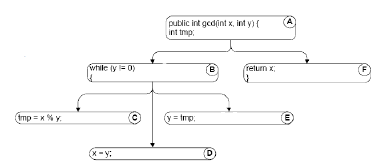
\includegraphics[scale = 0.7]{image/10.PNG}
%    \caption{Titre}
%    \label{fig:titre}
%\end{figure}

\section{Software Quality}
\textbf{\textit{Define aspects of software defects and defect management alternatives. Discuss different software quality characteristics and perspectives. Define correctness, reliability, safety and robustness.}}

\subsection{Define aspects of software defects and defect management alternatives}
\noindent \textbf{Defect} $=$ some problem with the software (Human error $\rightarrow$ Fault $\rightarrow$ Failure)
\begin{enumerate}
    \item $=$ \textbf{Error} : a mistake in performing some software activities
    \item $=$ \textbf{Fault} : a defect in the product
    \item $=$ \textbf{Failure} : a departure from the system's required behaviour
\end{enumerate}
\vspace{.5em}
\begin{enumerate}
    \item[$\Rightarrow$] \textit{High quality} $\approx$ low defect
    \item[$\Rightarrow$] \textit{Quality problem} $\approx$ defect impact
\end{enumerate}


\noindent \textbf{Dealing with defects : }
\vspace{-0.3cm}
\begin{multicols}{2}
\begin{enumerate}
    \item \textbf{Defect prevention} :
    \begin{itemize}
        \item [$\bullet$]Prevent faults from being injected
        \item [$\bullet$]Error blocking,
error source
removal
    \end{itemize}
    \item \textbf{Defect removal} :
    \begin{itemize}
        \item [$\bullet$]Remove faults
        \item [$\bullet$]Inspection
(find faults),
testing (find failures from faults
    \end{itemize}
    \item \textbf{Defect containment} :
    \begin{itemize}
        \item [$\bullet$]Keep failures local,
reduce failure impact
        \item [$\bullet$]Fault-tolerance,
failure containment
    \end{itemize}
\end{enumerate}
\columnbreak
\begin{center}
    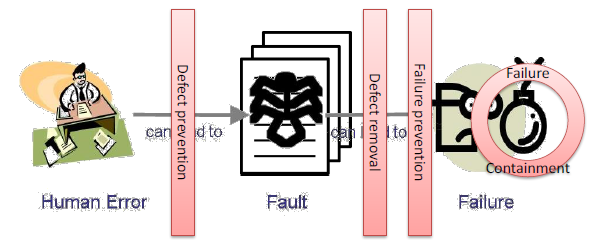
\includegraphics[scale = 0.5]{image/1.PNG}
\end{center}
\end{multicols}


\subsection{Discuss different software quality characteristics and perspectives}
\begin{enumerate}
    \item \textbf{Transcendental view} : Quality is an ideal that we thrive to but cannot attain
    \item \textbf{User view} : Quality
is
fitness
for
purpose,
reliability,
absence
of
defects
    \item \textbf{Manufacturing view} : Quality
is
conformance
to
the
process
    \item \textbf{Product view} : Quality
is
showing
good
inherent
characteristics
    \item \textbf{Value-based view} : Quality is how much the customer is willing to pay for it
\end{enumerate}
\vspace{0.3cm}
\noindent Quality
models
relate
the
user's
external
view
to
the
developer's
internal
view :

\begin{enumerate}
\item \textbf{Consumers} $=$
    \begin{enumerate}
        \item \textbf{Client} : pay for the development
        \item \textbf{User} of software
        \item \textbf{Customers} : buy  after development
    \end{enumerate}
    Expect \textbf{external} qualities : 
    \begin{enumerate}
        \item good enough for the price
        \item fit‐for‐use, doing the right things
        \item conformance, doing things right
    \end{enumerate}
    \item[$\Rightarrow$] \textbf{Judge external characteristics} : number and type of \textbf{failures}
    
    \item \textbf{Producers} $=$ Developer
    \\ Expect \textbf{internal} qualities : 
    \begin{enumerate}
        \item good enough for the cost
        \item maintainable
        \item interoperable
        \item modular
    \end{enumerate}
     \item[$\Rightarrow$] \textbf{Judge internal characteristics} : number and type of \textbf{faults}
\end{enumerate}

\noindent Quality characteristics (for customers) : 
\begin{enumerate}
    \item \textbf{Functionality} :\\
    A set of attributes that bears on the existence of a set of functions
and their specified properties. The functions are those that satisfy
stated or implied needs
    \item \textbf{Reliability} :\\
    A set of attributes that bears on the capability of software to
maintain its performance level under stated conditions for a stated
period of time
    \item \textbf{Usability} :\\
    A set of attributes that bears on the effort needed for use and on
the individual assessment of such use by a stated or implied set of
users
    \item \textbf{Efficiency} :\\
    A set of attributes that bears on the relationship between the
software performance and the amount of resources used under
stated conditions
    \item \textbf{Maintainability} :\\
    A set of attributes that bears on the effort needed to make specified
modifications (which may include corrections, improvements, or
adaptations of software to environmental changes and changes in
the requirements and functional specifications)
    \item \textbf{Portability} :\\
    A set of attributes that bears on the ability of software to be
transferred from one environment to another (including the
organizational, hardware, or software environment)
\end{enumerate}

\newpage
\subsection{Define correctness, reliability, safety and robustness}

\noindent These are "dependability properties" (Correctness
properties
are
\textbf{undecidable} for non-trivial programs): 
\begin{itemize}
    \item [$\bullet$]\textbf{Correctness:} a program is correct if it is consistent with its specification (seldom practical for non-trivial systems)
    \item [$\bullet$]\textbf{Reliability:} likelihood of correct function for some "unit" of behavior, relative to a specification and usage profile, statistical approximation to correctness (100\% reliable = correct)
    \item [$\bullet$]\textbf{Safety:} preventing hazards, which are system-specific undesirable behaviours
    \item [$\bullet$]\textbf{Robustness:} acceptable (degraded) behavior under extreme conditions
\end{itemize}
\begin{center}
    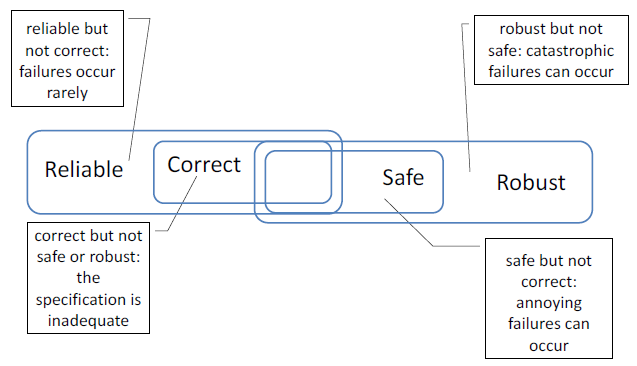
\includegraphics[scale = 0.55]{image/2.png}
\end{center}

\newpage
\section{Software development process}
\textbf{\textit{Define software verification and validation. Describe a software development process and how verification
and validation activities fit into this process. Describe different types of software quality assurance activities.}}

\subsection{Define software verification and validation}
\vspace{-0.5cm}
\begin{multicols}{2}
\begin{enumerate}
\item \textbf{Validation} $=$ does
the
software
system
meets
the
user's
real
needs? are
we building
the
right
software?
\begin{itemize}
    \item [$\Rightarrow$] specifications
accurately
reflects
the
customer's
needs\\
\end{itemize}
\textbf{Techniques : }
\begin{enumerate}
    \item Modeling
    \item Scenarios
    \item Prototypes
    \item Simulation
    \item  ...
\end{enumerate}
\vfill\null
\columnbreak
\item \textbf{Verification} $=$ does
the
software
system
meets
the
requirements
specifications? are
we building
the
software
right?
\begin{itemize}
    \item [$\Rightarrow$] application
conform
to
specifications\\
\end{itemize}
\textbf{Techniques : }
\begin{enumerate}
    \item Consistency/Completeness/Reachability checks 
    \item Model
checking
    \item Mathematical
proofs
\end{enumerate}
\end{enumerate}
\vfill\null
\end{multicols}

\vspace{-0.8cm}
\subsection{Describe a software development process and how verification
and validation activities fit into this process}
\noindent \textbf{Classic approach} : Requirement $\Rightarrow$ Specification $\Rightarrow$  Design $\Rightarrow$ Coding $\Rightarrow$ Testing $\Rightarrow$ Release

\noindent \textbf{Variation} : waterfall,
iterative,
spiral,
agile,
XP, ...

\begin{multicols}{2}
\begin{center}
    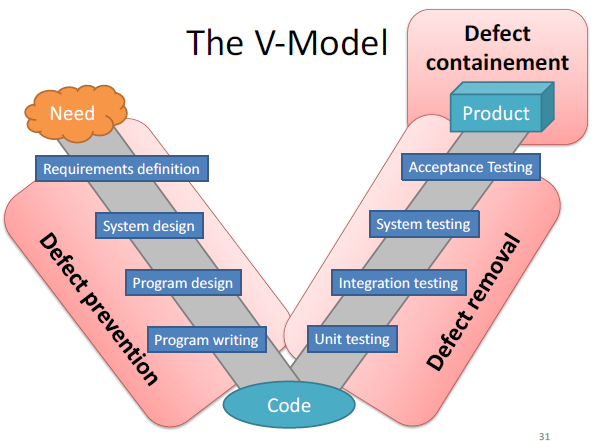
\includegraphics[scale = 0.4]{image/3.PNG}
\end{center}
\vfill\null
\columnbreak
\begin{center}
    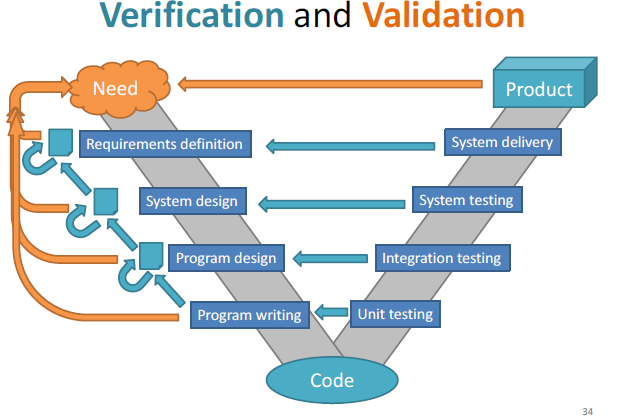
\includegraphics[scale = 0.4]{image/4.PNG}
\end{center}
\end{multicols}
\vspace{-1.2cm}
\subsection{Describe different types of software quality assurance activities}
\begin{enumerate}
    \item \textbf{Testing : }
    \begin{itemize}
        \item [$\bullet$]Executed
late
in
development
        \item [$\bullet$]Start
as
early
as
possible
        \item [$\bullet$]Early
test
generation
has
several
advantages
        \begin{enumerate}
            \item Tests
generated
independently
from
code,
when
the
specifications
are
fresh
in
the
mind
of
analysts
            \item The
generation
of
test
cases
may
highlight
inconsistencies
and
incompleteness
of
the
corresponding
specifications
            \item tests
may
be
used
as
compendium
of
the
specifications
by
the
programmers
        \end{enumerate}
    \end{itemize}
    \item \textbf{Inspection : }
    \begin{itemize}
        \item [$\bullet$]can
be
applied
to
essentially
any
document
        \begin{enumerate}
            \item requirements
statements
            \item architectural
and
detailed
design
documents
            \item test
plans
and
test
cases
            \item program
source
code
        \end{enumerate}
        \item [$\bullet$]may
also
have
secondary
benefits
         \begin{enumerate}
            \item spreading
good
practices
            \item instilling
shared
standards
of
quality
        \end{enumerate}
        \item [$\bullet$]takes
a
considerable
amount
of
time
        \item [$\bullet$]re-inspecting
a
changed
component
can
be
expensive
        \item [$\bullet$]used
primarily
         \begin{enumerate}
            \item where
other
techniques
are
inapplicable
            \item where
other
techniques
do
not
provide
sufficient
coverage\\
        \end{enumerate}
    \end{itemize}
    \item \textbf{Automatic Static Analysis : }
    \begin{itemize}
        \item [$\bullet$]More
limited
in
applicability
\begin{enumerate}
    \item can
be
applied
to
some
formal
representations
of
requirements
models
    \item not
to
natural
language
documents
\end{enumerate}
        \item [$\bullet$]Are
selected
when
available
        \begin{enumerate}
    \item substituting
machine
cycles
for
human
effort
makes them
particularly
cost-effective\\
\end{enumerate}


    \end{itemize}
        \item \textbf{Computer-Aided
Verification : }
    \begin{itemize}
        \item [$\bullet$]\textbf{Model
checking:} exhaustive
search
of
a
specification's
execution
space
\begin{enumerate}
    \item applicable
to
behavior models
(e.g.
statecharts,
Petri
nets)
    \item check
state
conditions,
temporal
logic,
compare
models
\end{enumerate}
        \item [$\bullet$]\textbf{Theorem
proving:} prove
Specifications AND
Assumptions IMPLY
Requirements
        \begin{enumerate}
    \item using
built‐in
theories,
inference
rules,
decision
procedures\\
\end{enumerate}

    \end{itemize}
     \item \textbf{Improving the
Process : }
    \begin{itemize}
        \item [$\bullet$]Long
lasting
errors
are
common

        \item [$\bullet$]It
is
important
to
structure
the
process
for
        \begin{enumerate}
    \item the
most
critical
persistent
faults
    \item tracking
them
to
frequent
errors
    \item adjusting
the
development
and
quality
processes
to
eliminate
errors
\end{enumerate}
        \item [$\bullet$]Feedback
mechanisms
are
the
main
ingredient
of
the
quality
process
for
identifying
and
removing
errors

    \end{itemize}
\end{enumerate}



\newpage
\section{Behaviour models}
\textbf{\textit{Define state models. Describe control flow graphs and their constituents. Describe call graphs and discuss context-sensitive analysis. Describe finite state machines and discuss abstraction.}}

\subsection{Define state models}
\vspace{-0.5cm}
\begin{multicols}{2}
\begin{itemize}
    \item [$\bullet$]\textbf{Models} = \textbf{abstraction} of the system (removes irrevelant attributes or details via an abstraction function)
    \begin{itemize}
        \item [$\blacksquare$]Represent a system, an artifact, a design

        \item [$\blacksquare$]Analyse a system, an artifact, a design
        \begin{itemize}
            \item before the system is built
            \item easier to analyse/check/test than the actual system
        \end{itemize}
    \end{itemize}
    \textbf{Properties} : Compact, Predictive, Semantically meaningful and Sufficiently general
    
    \vfill\null
    \columnbreak
    \item [$\bullet$]\textbf{State models}  \\ \textbf{Program execution} = sequence of states and transitions
    \begin{itemize}
        \item [$\blacksquare$]\textbf{States} : control + data (Location + variables, stack, heap)

        \item [$\blacksquare$]\textbf{Transitions}: actions (ops, instructions)
    \end{itemize}
    \textbf{State Space} :
    \begin{itemize}
        \item [$\blacksquare$]\textit{Full} (all possible values)
        \item [$\blacksquare$]\textit{Reachable} (from initial states)
    \end{itemize}
    Essentially \textbf{infinite}. \\
    \textbf{Finite models} of program execution \\$\Rightarrow$ abstraction
    \begin{enumerate}
        \item Execution is \textbf{coarsened} (fewer steps)
        \item \textbf{Nondeterminism} is introduced
    \end{enumerate}
    \vfill\null
\end{itemize}
\end{multicols}
\vspace{-0.9cm}


\subsection{Describe control flow graphs and their constituents}
\noindent \textbf{Abstraction} : set of program locations (PC) $\rightarrow$ finite number of locations

\begin{multicols}{2}
\noindent \textbf{Control Flow Graph (CFG)} :
\begin{itemize}
    \item [$\bullet$]\textbf{Nodes} = regions of source code (basics blocks)
    \begin{itemize}
        \item[$\blacksquare$] Basic block: maximal program region with a single entry and single exit point
        \begin{enumerate}
            \item Often several statements in one blocks
            \item Sometimes one statement in several blocks
        \end{enumerate}
    \end{itemize}
    \item [$\bullet$]\textbf{Edge} = possibility that execution proceeds from the end of one region to the beginning of another
\end{itemize}

    \vfill\null
    \columnbreak

\begin{center}
    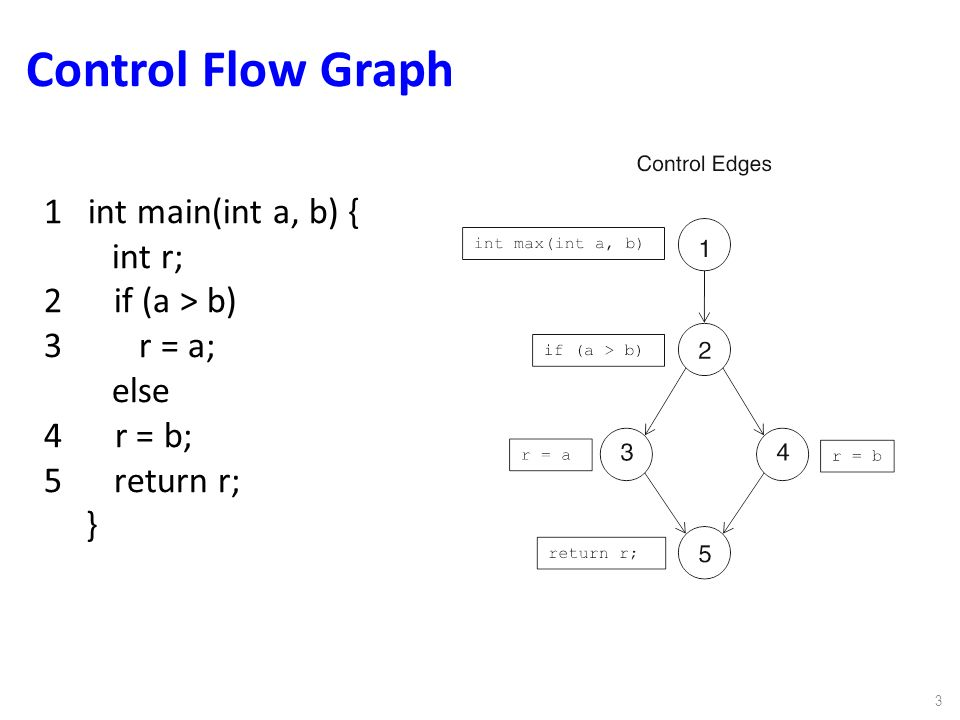
\includegraphics[scale=0.3]{image/1.jpg}
\end{center}
\end{multicols}


\noindent $\Rightarrow$\textbf{Intra-procedural} (ignore calls). May not cover some flows (e.g : exceptions are not covered)
\vspace{3em}

\noindent\textbf{Linear Code Sequence and Jump (LCSJ)}:\\
Subpaths from
one
branching
point
to
another
(jumps)
proceeding
to
next
block
is
not
branching

\newpage
\subsection{Describe call graphs and discuss context-sensitive analysis}
\noindent Call graphs : 
\begin{itemize}
    \item [$\bullet$]Nodes represent procedures
    \item [$\bullet$]Edges represent calls relation\\
\end{itemize}
\noindent $\Rightarrow$\textbf{Inter-procedural} 

\begin{figure}[h!]
\centering
\begin{subfigure}{.5\textwidth}
  \centering
        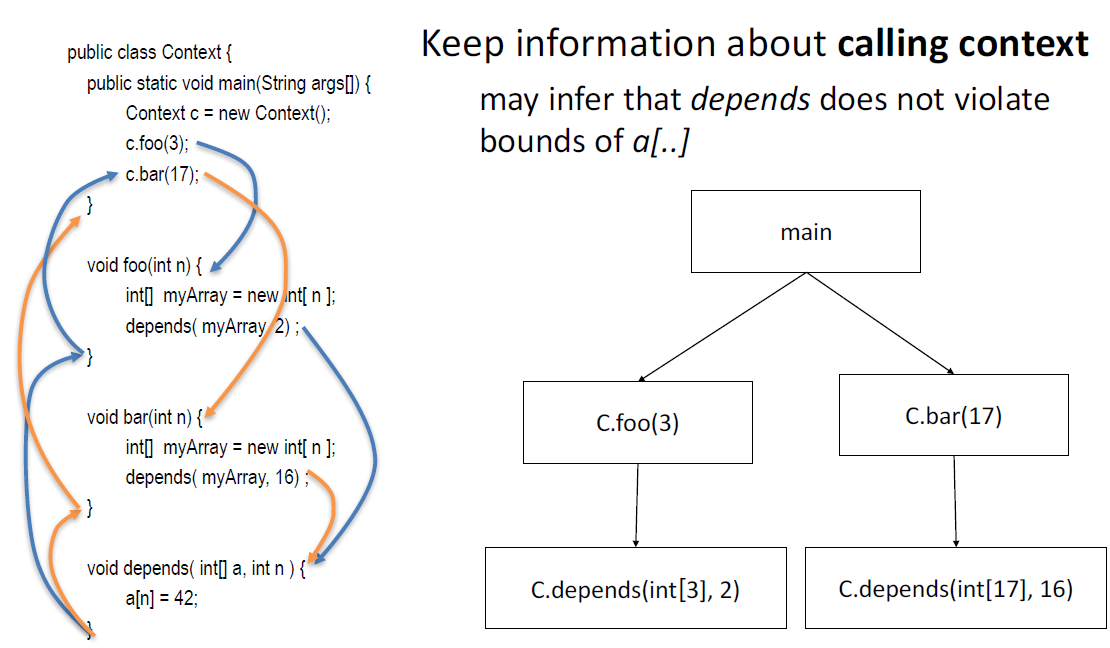
\includegraphics[width=1\linewidth]{image/5.PNG}
  \caption{Context-sensitive}
  \label{fig:sub1}
\end{subfigure}%
\begin{subfigure}{.5\textwidth}
  \centering
        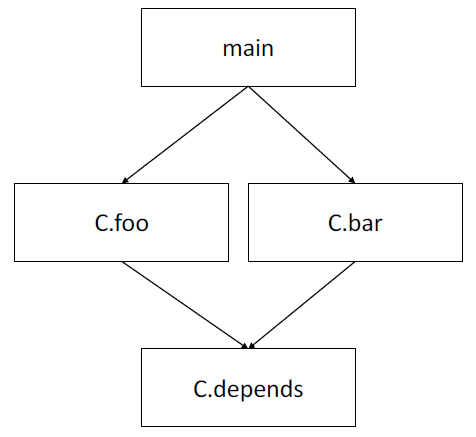
\includegraphics[width=0.5\linewidth]{image/6.PNG}
  \caption{Context-insensitive}
  \label{fig:sub2}
\end{subfigure}
\label{fig:test}
\end{figure}

\noindent\textbf{Context-sensitive analysis}:  the number of contexts grows exponentially with the depth of the calls.
\begin{itemize}
    \item [$\bullet$] $\#C \approx \#P^{depth}$   : where $\#C =$ number of contexts and $\#P =$ number of procedures

\end{itemize}

\newpage
\subsection{Describe finite state machines and discuss abstraction}

\begin{itemize}
    \item [$\bullet$]\textbf{Nodes} = states (finite number)
    \item [$\bullet$]\textbf{Edges} = transitions
    \begin{itemize}
        \item [$\blacksquare$]labelled with condition, operation, event
        \item [$\blacksquare$]input/output : Mealy Machine
    \end{itemize}
    \item[$\Rightarrow$]Used as \textbf{specifications} of allowed behaviour
\end{itemize}

\noindent For example, a transition diagram (Mealy machine) or a state-transition table.\\

\noindent\textbf{Abstraction function}: checking correctness with respect to the written program (Finite State Machine accurately represents program behaviour $\equiv$ program correctly implements FSM abstraction).\\
\textbf{Abstract} (function): takes a program state returns a FSM state\\

\noindent \textbf{Example : }
\begin{center}
    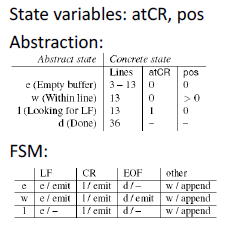
\includegraphics[scale = 0.7]{image/7.PNG}
\end{center}

\newpage
\section{Data models}
\textbf{\textit{Define data dependence based on def-use pairs. Describe data dependence and control dependence graphs. Explain the general principle of dataflow analyses based on worklist algorithms, and the particular case of computing reaching definitions. Discuss the effect of pointers and procedures.}}

\subsection{Define data dependence based on def-use pairs}
\begin{multicols}{2}
\begin{enumerate}
    \item \textbf{def} :\\
    Point where a variable gets a value\\
    (declaration, initialization, assignment or value received by parameter)
    \item \textbf{use} :\\
    Point where a value from a variable is used\\
    (expression, conditional statement, parameter passing, returns)
    \item[$\Rightarrow$] \textbf{def-use pair} : pair of points
    \begin{itemize}
        \item [$\bullet$]from where a value is produced
        \item [$\bullet$]to where that value is used
    \end{itemize}
\end{enumerate}
\vfill\null
\columnbreak
\begin{center}
    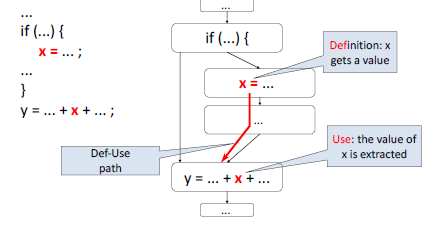
\includegraphics[scale = 0.8]{image/8.PNG}
\end{center}
\end{multicols}
\noindent$\Rightarrow$ \textbf{Data dependence based on def-use pairs}: Where does this value of x come from? What would be affected by changing this? ...


\subsection{Describe data dependence and control dependence graphs}
\vspace{-0.5cm}
\begin{multicols}{2}
\noindent \textbf{Data dependence graph} :
\begin{enumerate}
    \item \textbf{Nodes} : \\Program regions as in the control flow graph
    \item \textbf{Edges} : \\\textbf{Def-use pairs} labelled with the variable name
    \item[$\Rightarrow$] \textbf{Data dependence} :\\ P2 depends on P1 iff data values used in P2 can be defined in P1 (P1 is a \textbf{definition point}, P2 is an \textbf{use point})
\end{enumerate}
\vfill\null
\begin{center}
    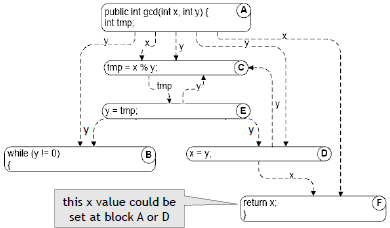
\includegraphics[scale = 0.7]{image/9.PNG}
\end{center}
\columnbreak
\noindent \textbf{Control dependence graph} :
\begin{enumerate}
    \item \textbf{Nodes} : \\Program regions as in the control flow graph
    \item \textbf{Edges} : \\from \textbf{entry/branching} points to controlled blocks
    \item[$\Rightarrow$] \textbf{Control dependence}: \\P2 depends on P1 iff P1 controls whether P2 executes (P1 is an \textbf{entry/branching point}, P2 is \textbf{any point})
\end{enumerate}

\vfill\null
\begin{center}
    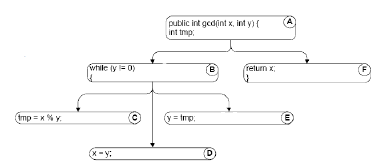
\includegraphics[scale = 0.7]{image/10.PNG}
\end{center}
\end{multicols}
The difference with control flow is that blocks of CFG only follow other blocks but do not depends on them. Either of these blocks could be executed in either order.

\subsection{Explain the general principle of dataflow analyses based on worklist algorithms, and the particular case of computing reaching definitions}
\vspace{-0.5cm}
\begin{multicols}{2}
\noindent Let :
\begin{enumerate}
    \item $v_d, v_e$ definitions of variables $v$ at points $d,e$
    \item $u$ a point where $v$ is used
    \item[$\Rightarrow$]definition $v_d$ \textbf{reaches} $u$ ($v_d$ is a \textbf{reaching definition} at $u$) iff 
    \begin{enumerate}
        \item There is at least one control flow path from $d$ to $u$
        \item There is no intervening definition of $v$ on the path
    \end{enumerate}
    \item[$\Rightarrow$]$v_e$ \textbf{kills} $v_d$ iff it is on a control path from $d$
    \item[$\Rightarrow$]$(d,u)$ is a \textbf{def-use pair} of $v$ iff $v_d$ \textbf{reaches} $u$
\end{enumerate}
\columnbreak
\vfill\null
\begin{center}
    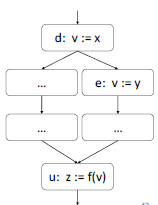
\includegraphics[scale = 0.8]{image/11.PNG}
\end{center}
\end{multicols}

\noindent \textbf{Calculating Def‐Use
Pairs} : \\
Even with loop‐free paths, the number of paths in a graph can be \textbf{exponentially larger} than the number of nodes and edges. So we don’t want to search every individual path but we
want to summarize the reaching definitions at a node over all the paths reaching that node.
\begin{multicols}{2}
\noindent \textbf{DF Algorithm} :
\begin{itemize}
    \item [$\bullet$]\textbf{Goal}: compute reaching definitions at node $n$
    \item [$\bullet$]Suppose that node $p$ is an immediate predecessor of node $n$
    \begin{itemize}
        \item If $p$ can assign var. $v$, then $v_p$ reaches $n$.\\We say the definition $v_p$ is generated at $p$
        \item If a definition $v_d$ reaches $p$, and if $v$ is not redefined at $p$, then $v_d$ reaches $n$.
    \end{itemize}
    \item [$\bullet$]$Reach(n) =$ set of definitions that reach $n$
    \item [$\bullet$]$ReachOut(n) =$ set of definitons that exit $n$
\end{itemize}
\columnbreak
\vfill\null
\textbf{Recursive equations} for
all nodes n\\
\textbf{Fixed point} computation
\begin{center}
    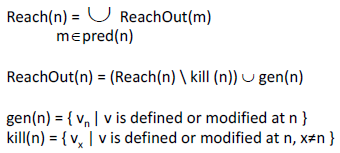
\includegraphics[scale = 0.8]{image/12.PNG}
\end{center}
\vfill\null
\end{multicols}

\noindent \textbf{Worklist
Algorithm} :
\begin{lstlisting}[escapeinside={(*@}{@*)}]
foreach n (*@$\in$@*) nodes {
    ReachOut(n) = {}
}
worklist = nodes
while worklist (*@$\neq$@*) {} {
    n = choose(worklist)
    worklist = worklist\{n}
    oldVal = ReachOut(n);
    Reach(n) = (*@$\bigcup_{m \in pred(n)}$@*) ReachOut(m)
    ReachOut(n) = (Reach(n)\kill(n)) (*@$\cup$@*) gen(n)
    if ReachOut(n) (*@$\neq$@*) oldVal {
        worklist = worklist (*@$\cup$@*) succ(n)
    }
}
\end{lstlisting}

\noindent \textbf{Example} :
\begin{center}
        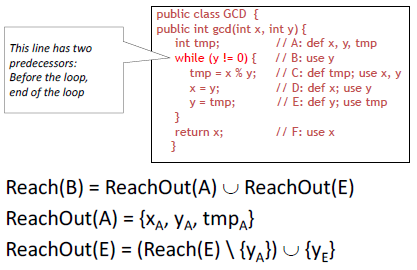
\includegraphics[scale = 0.7]{image/13.PNG}
\end{center}

\vspace{-0.5cm}
\noindent \textbf{Particular cases} :
\begin{enumerate}
    \item \textbf{Avail expressions} : expression exp is \textbf{available} at node n iff for all paths to n, exp has been computed and not subsequently modified (used in compiler construction)
\begin{center}
        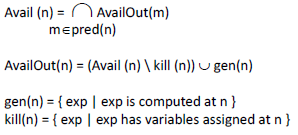
\includegraphics[scale = 0.7]{image/14.PNG}
\end{center}
    \item \textbf{Live variables} : A variable v is \textbf{live} at node n iff on some execution path from n, v is used before it is changed
\begin{center}
        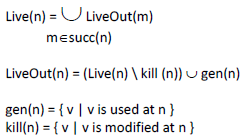
\includegraphics[scale = 0.7]{image/15.PNG}
\end{center}
\end{enumerate}
\vspace{-0.5cm}
\noindent \textbf{Classification of
analyses} :
\begin{itemize}
    \item [$\bullet$]\textbf{Forward/backward:}
a
node’s set
depends on
that of
its
predecessors/successors
    \item [$\bullet$]\textbf{Any-path/all‐path}:
a
node’s set
contains a
value iff it is coming
from
any/all of
its inputs
\end{itemize}
\begin{center}
        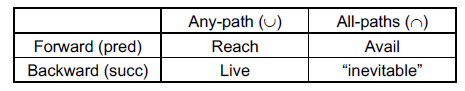
\includegraphics[scale = 0.6]{image/16.PNG}
\end{center}

\newpage
\subsection{Discuss the effect of pointers and procedures}
\begin{enumerate}
    \item \textbf{Arrays and pointers} : introduce \textbf{uncertainty}: do different expressions access the same storage? \\For example: a[i] is the same as a[k] when i=k or a[i] same as b[i] when a=b. 
    
    \textbf{Solution}: 
    \begin{enumerate}
        \item \textbf{Any-path}: gen sets contains all potential aliases, kill sets contain only what is definitely modified.
        \item \textbf{All-path}: vice versa\\
    \end{enumerate}
    \item \textbf{Procedures} : \textbf{interprocedural} (Across several methods or procedures) data flow analysis has critical and difficult cost/precision trade-offs: context sensitivity and flow sensitivity. \\For example: Reach, Avail,... are flow-sensitive and \textbf{intraprocedural} (Within
a
single
method
or
procedure) analyses which cost $O(n^3)$ for one procedure (reasonably cheap) but what about doing flow-sensitive interprocedural analyses? $\rightarrow$ $O(n^3)$ on the whole program : prohibitive ! So, many interprocedural flow analyses are flow-insensitive (it is often good enough, e.g. type checking)
\end{enumerate}


\newpage
\section{Functional testing}
\textbf{\textit{Define test case, test obligation, adequacy criterion, test satisfaction. Define functional and structural testing. Explain category-partition testing. Explain pair-wise and n-wise testing. Explain catalog-based testing.}}

\subsection{Define test case, test obligation, adequacy criterion, test satisfaction}
\vspace{-0.5cm}
\begin{multicols}{2}
\begin{enumerate}
    \item \textbf{Test case} :\\
    a set of inputs, execution conditions, and a pass/fail criterion for judging test execution
    \\
    \item \textbf{Test case specification} :\\
    a requirement to be satisfied by one or more test cases\\
    \item \textbf{Test obligation} :\\ 
    a partial test case specification, requiring some property deemed (= considered) important to thorough testing
    \vfill\null\columnbreak
    \item \textbf{Adequacy criterion}:\\ 
    a predicate that a <program, test suite> pair must satisfy; usually expressed in the form of a rule for deriving a set of test obligations from another artifact (program, specification)\\
    \item \textbf{Test satisfaction}:\\ 
    A test suite (set of test cases) satisfies an adequacy criterion if:
    \begin{itemize}
        \item [$\bullet$]all the tests succeed (pass)
        \item [$\bullet$]every obligation is satisfied by at least one test case
    \end{itemize}
    \vfill\null
\end{enumerate}
\end{multicols}
\vspace*{-0.5cm}
\noindent\textbf{Infeasible Criterion}: Sometimes
no test
suite
can
satisfy
a
criterion
for
a
given
program 
\begin{itemize}
    \item [$\Rightarrow$]Solution:
eliminate infeasible
test
obligations = \textbf{Undecidable
in
the
general
case!}
    \item [$\Rightarrow$]\textbf{Solution}:
measure fraction
of
obligations
covered = \textbf{Coverage}
\end{itemize}
%\vspace*{-1.5cm}
\subsection{Define functional and structural testing}
\vspace{-0.5cm}
\begin{multicols}{2}
\begin{enumerate}
    \item \textbf{Functional testing} : (black box, closed box)
    \begin{itemize}
        \item [$\bullet$]Program content is unknown or ignored
        \item [$\bullet$]Test input/output behavior
        \item [$\bullet$]Obligations from functional specifications (informal textual specs, tables, state graphs, UML, ...)
        \item [$=$] \textbf{systematic testing} (select inputs that are especially valuable, different classes, limit cases, special values)
    \end{itemize}
    \vfill\null\columnbreak
    \item \textbf{Structural testing} : (white box, clear box)
    \begin{itemize}
         \item [$\bullet$]Program content is visible and observed $\rightarrow$ example : if test suite executes all program statements/conditions/branches/..., then coverage is 100\%
         \item [$\bullet$]Test internal operation
         \item [$\bullet$]Obligations from program code
     \end{itemize}
 \vfill\null
\end{enumerate}
\end{multicols}

\newpage
\subsection{Explain category-partition testing}
\noindent\textbf{Category-partition testing} : 3 steps
\begin{enumerate}
    \item \textbf{Decompose the specification into units, parameters, categories}
    \begin{enumerate}
        \item Identify independently testable units
        \item For each unit, identify parameters and environment elements
        \item For each parameter, identify categories (characteristics) → Not a trivial task ! No
hard-and-fast rules, reflect test designer’s judgment,...\\
    \end{enumerate}
    \item \textbf{Identify relevant choices (values) for each category}
    \begin{enumerate}
        \item Identify classes of values for each category (ignore interactions
between different categories)

        \item Boundary value testing
        \begin{enumerate}
            \item extreme values within a class
            \item values just outside the class
            \item interior (non-extreme) values
        \end{enumerate}
        \item Erroneous condition testing : values outside the normal domain of the program\\

    \end{enumerate}
    \item  \textbf{Introduce constraints} : combination of values for each category corresponds to a test case specification. Number of combinations = product of category sizes, most of which are impossible ! Introduce constraints to rule out impossible combinations, or to reduce the size of the test suite if too large
\end{enumerate}

\subsection{Explain pair-wise and n-wise testing}
Category-partition testing is a systematic approach to generate combinations, but the test suite
size grows very rapidly with the number of categories, even with constraints! The idea of pairwise
testing is to use a non-exhaustive approach
\begin{enumerate}
    \item \textbf{Pair-wise testing} : all \textbf{pairs of choices}\\
    \textbf{Pairwise combination} : generate combinations that efficiently cover all pairs (triples,... in case of n-wise) of choices. Justified by the fact that most failures are triggered by a single value or a combination of a few values, so covering pairs (triples,...) reduces the number of test cases, but reveals most faults.\\
    \textbf{Complexity} : For N categories with M choices each :
    \begin{itemize}
        \item [$\bullet$]\textbf{All combinations} $= O(M^N)$ test cases → exponential in number of categories
        \item [$\bullet$]\textbf{All pairs} $= O(M^2  log(N))$ test cases → logarithmic in number of categories\\
    \end{itemize}
    
    \item \textbf{N-wise testing} : same as pairwise but for all N-uples of choices
\end{enumerate}

\newpage
\subsection{Explain catalog-based testing}
\begin{itemize}
    \item [$\bullet$]Deriving value classes requires human judgment, catalog-based testing aims to gather experience in a systematic collection
    \item [$\bullet$]Catalogs list important cases for each possible type of variable
    \begin{multicols}{2}
    \item [$\bullet$]\textbf{Benefits} :
    \begin{enumerate}
        \item speed up the test design process
        \item routinize many decisions, better focusing human effort
        \item accelerate training and reduce human error
    \end{enumerate}
    \vfill\null\columnbreak
    \item [$\bullet$]\textbf{Process} :
    \begin{enumerate}
        \item analyze the initial specification to identify simple
elements : pre-conditions, post-conditions, definitions,
variables, operations

        \item derive a first set of test case specifications from pre-conditions, post-conditions
and definitions
        \item complete the set of test case specifications using test catalogs
    \end{enumerate}
    \end{multicols}
\end{itemize}

\noindent \textbf{Catalog}:
\begin{enumerate}
    \item Each
entry
=
a
kind
of
element
that
can
occur
in
a
specification
    \item Each
entry
is
associated
with
a
list
of
generic
test
case
specifications\\
\end{enumerate}

\noindent \textbf{Example}:\\
Catalog entry \textit{Boolean}\\
Two test case specifications: \textit{true}, \textit{false}\\
Label in/out indicate if applicable only to \textit{input}/\textit{output} or \textit{both}

\begin{center}
        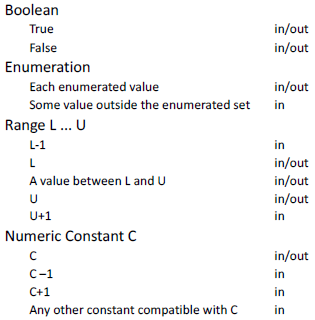
\includegraphics[scale = 0.8]{image/17.PNG}
\end{center}

\newpage
\section{Structural testing}
\textbf{\textit{Define statement, branch and condition coverage, compound conditions and MC/DC, and compare their strengths. Define
path coverage, discuss limitations and show some practical path coverage
criteria. Define data flow coverage criteria. Discuss the problems of aliases
and infeasibility.}}

\subsection{Define statement, branch and condition coverage, compound conditions and MC/DC, and compare their strengths}
\vspace{-0.5cm}
\begin{multicols}{2}
\begin{enumerate}
    \item \textbf{Statement coverage} : \\ 
    each statement must be executed at least once. Motivation: a fault in a statement can only be revealed by executing the faulty statement 
    $$C_{stmt} = \frac{\#executed\;statement}{\#statement}$$
    NB : CFG nodes $\neq$ statements : may represent basic blocks, multiple statements or parts of statements. Difference in granularity, not in concept. 100\% node coverage = 100\% statement coverage\\
    \item \textbf{Branch coverage} :\\ each branch must be executed at least once. Variant: edge coverage → each edge in the CFG. In a graph: traversing all edges $\Rightarrow$ visiting all nodes.
    $$C_{branch} = \frac{\#executed\;branches}{\#branches}$$
    NB: 100\% branch coverage $\Rightarrow$ 100\% statement coverage (but not the converse!)\\
    Branch coverage = \textbf{decision coverage} : each decision must be true and false at least once (decision =
    top-level boolean expression)\\
    %\vfill\null\columnbreak
    \item \textbf{Condition coverage}:\\ 
    considers case analysis in more detail : individual conditions in a boolean decision are tested. Each \textbf{basic condition} must be true and false at least once.
$$C_{bcond} = \frac{
\begin{gathered}
\#executed\;true\;basic\;conds\\
+\#executed\;false\;basic\;conds
\end{gathered}
}{2*\#basic\;conds}$$
    Note: basic condition coverage can be satisfied without satisfying branch
coverage. Branch and basic condition are not comparable → neither implies the other\\
    \item \textbf{Compound conditions coverage}:\\ 
    each possible evaluation of each decision must be taken at least
once: all branches of the decision tree.
Note : exponential complexity. N conditions $\Rightarrow$ $O(2^N)$ test cases
\begin{center}
 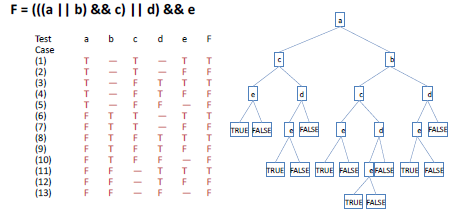
\includegraphics[scale=0.6]{image/18.PNG}   
\end{center}

     %\vfill\null\columnbreak
     \item \textbf{MC/DC (Modified condition/decision) coverage}:\\
     each basic condition is
shown to independently affect the decision\\
\textbf{Motivation}: test important combinations of conditions, without
exponential blowup \\
Requires, for each basic condition C in a decision D, two test cases
such that:
\begin{enumerate}
    \item Values of all evaluated conditions except C are the same
and 
    \item D evaluates to true for one and false for the other
\end{enumerate}
\begin{center}
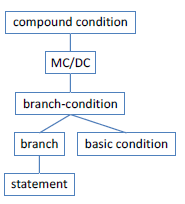
\includegraphics[scale=0.8]{image/20.PNG}
\end{center}
N basic conditions $\Rightarrow$ N+1 test cases (linear complexity)
\begin{center}
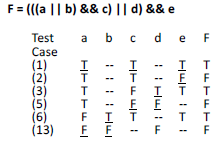
\includegraphics[scale=0.8]{image/19.PNG}
\end{center}
It is a good balance of thoroughness and test size (and therefore widely
used).\\

It is basic condition coverage (C) + decision (=branch) coverage (DC) + one additional condition (M) that every condition must independently affect the decision’s output.
\end{enumerate}
\end{multicols}
%\vspace*{-0.8cm}

\subsection{Define
path coverage, discuss limitations and show some practical path coverage
criteria}
\begin{multicols}{2}
\begin{itemize}
    \item[$\bullet$] \textbf{Path coverage} : decision and condition coverage only consider individual program decisions. Many more paths than branches. Each path must be executed at least once
    $$C_{path} = \frac{\#executed\;paths}{\#paths}$$
    \item[$\bullet$] \textbf{Limitations} :
     \begin{enumerate}
         \item Program with loops $\Rightarrow$ infinite number of paths ! Full path coverage is therefore usually
impossible to satisfy.
        \item Feasible criterion : partition infinite set of paths into a finite number of classes, by limiting:
        \begin{enumerate}
            \item the number of traversals of loops
            \item the length of the paths to be traversed
            \item the dependencies among selected paths
        \end{enumerate}
       
     \end{enumerate}
    \vfill\null\columnbreak
    \item[$\bullet$] \textbf{Some practical path coverage criteria} : 
    \begin{itemize}
    \item [$\bullet$] \textbf{Boundary interior path coverage}: each path up to the first repeated node must be executed at least once
         \begin{enumerate}
            \item Group together paths that differ only in the subpath they follow when repeating the body of a loop
            \item construction: unfold the CFG up to the first repeated node
            \item limitations: the number of paths can still grow exponentially
        \end{enumerate}
    \item [$\bullet$]\textbf{Cyclomatic coverage}: a basis of independent paths must be executed
         \item [$\bullet$]\textbf{Loop boundary coverage}: each loop body must be iterated zero times, one time and more than
one time at least once.
     \end{itemize}
 \vfill\null
\end{itemize}
\end{multicols}
\vspace{-1cm}
\subsection{Define data flow coverage criteria}
\begin{enumerate}
    \item\textbf{Motivation for data flow testing} (not really asked) : statement and branch coverage don’t test interactions, path-based coverage require impractical number of test cases and only a few paths uncover additional faults. → We need to distinguish important paths. Intuition: statements interact through data flow (value computed in one statement, used another. Bad value computation revealed only when it is used)

    \item \textbf{All DU (def-use) pairs}: each DU pair is exercised at least once
    \item \textbf{All DU paths} : each simple (non looping) DU path is exercised at least once
    \item \textbf{All definitions}: for each definition, some DU pair is exercised at least once (every computed value
is used somewhere)
\end{enumerate}

\newpage
\subsection{Discuss the problems of aliases and infeasibility}
\begin{itemize}
    \item [$\bullet$]\textbf{Problem with aliases}: which references are (always or sometimes) the same?\\
Ex: p=\&x; ...; *p=99 → *p is an alias of x\\
    \item [$\bullet$]\textbf{Problem of infeasibility}: with conditional statement, it is possible that a variable is defined and
never used = infeasibility problem. This problem is relevant, combinations of elements matter, it is
impossible to decide feasible paths. In practice, we achieve reasonable coverage, but full
coverage is usually unattainable. Number of paths is exponential in worst case, but often linear.
But testing all DU paths is more often impractical since attainability is an undecidable problem
\end{itemize}


\newpage
\section{Model-based testing}
\textbf{\textit{Explain the principles of model-based testing. Explain path-insensitive and path-sensitive state machine coverage criteria. Discuss coverage criteria for decision structures and grammars.}}

\subsection{Explain the principles of model-based testing}
\begin{enumerate}
    \item It is used in order to test structured specifications (state machines, tables, graphs, grammars,...)
    \item Consist on devising test cases to check actual behavior against behavior specified by the model
    \item Coverage similar to structural testing, but applied to specification and design model
\end{enumerate}

\subsection{Explain path-insensitive and path-sensitive state machine coverage criteria}
\begin{enumerate}
    \item \textbf{Covering finite state machine} :\\
    Finite state machines: for describing behavior that depends on sequences of events or stimuli
    \begin{itemize}
        \item [$\bullet$]\textbf{State coverage}: every state in the model should be visited at least once
        \item [$\bullet$]\textbf{Transition coverage}: every transition in the model should be traversed at least once (this is the most commonly used criterion).\\
        Transition coverage assumes that \textbf{transitions depend only on current state} and not on path to reach the state. This is not always true → needs path-sensitive criteria
    \end{itemize}
    \item \textbf{Path-sensitive criteria} :
    \begin{itemize}
        \item [$\bullet$]\textbf{Single state path coverage}: traverse each subpath that reached states at most once
        \item [$\bullet$]\textbf{Single transition path coverage}: traverse each subpath that reaches transitions at most once
        \item [$\bullet$]\textbf{Boundary interior loop coverage}: traverse each distinct loop the minimum, an intermediate, and
the maximum or a large number of times (the most common)
    \end{itemize}
\end{enumerate}

\subsection{Discuss coverage criteria for decision structures and grammars}
\begin{itemize}
        \item [$\bullet$]\textbf{Coverage criteria for decision structures }: \\
        A representation of a function $result = F(conditions)$\\
        n conditions $\rightarrow$ $2^n$ possible combinations (decision tables/trees, flow charts).\\
        Treat as \textbf{Boolean expressions}.\\
        \textbf{Covering} : Apply condition/decision‐based criteria : 
        \begin{enumerate}
            \item \textbf{Basic condition coverage}: a test case for each column
            \item \textbf{Compound condition coverage}: a test case for each (possible) combination of basic conditions
            \item \textbf{Modified coverage (MC/DC)}: add columns that differ in one input row and in outcome, merge compatible columns, a test case specification for each column \\
        \end{enumerate}
        
        \item [$\bullet$]\textbf{Coverage criteria for decision grammars }: \\
        Useful for sequences and nested structure. Test cases are string generated from the grammar : 
        \begin{enumerate}
            \item \textbf{Production coverage}: each production must be used at least once
            \item \textbf{Boundary condition coverage}: each recursive production must be used (min, min+1, max-1, max) times, where min and max are set for each production (similar to boundary interior path)
        \end{enumerate}
        Test cases generated depend on generation strategy:
        \begin{enumerate}
            \item productions with non-terminals first → few, large test cases
            \item productions with terminals first → many, small test cases

        \end{enumerate}
\end{itemize}


\newpage
\section{Object-oriented testing}
\textbf{\textit{Explain the principles of testing of object-oriented software, at the unit and integration level. Discuss structural coverage criteria for intra- and inter-class testing. Discuss the issues of test oracles, polymorphism and exception handling.}}

\subsection{Explain the principles of testing of object-oriented software, at the unit and integration level}
\noindent For an object oriented software: \textbf{unit} = single class (or cluster of strongly related classes e.g. exceptions)
\begin{itemize}
    \item [$\Rightarrow$]\textbf{unit testing} = intra-class testing
    \item [$\Rightarrow$]\textbf{integration testing} = inter-class testing
\end{itemize}

\subsection{Discuss structural coverage criteria for intra- and inter-class testing}
\vspace{-0.5cm}
\begin{multicols}{2}
\begin{itemize}
    \item [$\bullet$]\textbf{Inter-class testing} (state machine):
    \begin{itemize}
        \item  Test interactions between classes
        \item Bottom-up integration, according to “depends”
relation
        \item Use/include hierarchy:
        \begin{enumerate}
            \item A uses B = A makes method calls on B
            \item A includes B = A objects include references to B objects, ignore inheritance, abstract
classes
        \end{enumerate}
        \item Bottom-up integration, clustering\\
    \end{itemize}
    
    %\vfill\null\columnbreak
    \item [$\bullet$]\textbf{Intra-class testing} :\\
    Basic idea:
    \begin{itemize}
        \item Objects have a state
        \item Methods calls are state transitions
        \item Test cases are sequences of method calls
    \end{itemize}
    State machine can be derived from specification and code → Model-based testing, state/transition coverage
    \begin{center}
    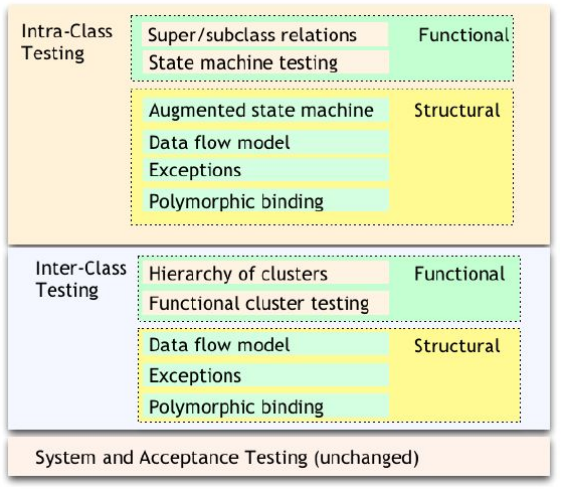
\includegraphics[scale = 0.4]{image/21.PNG}
\end{center}
    \vfill\null\columnbreak
    \item [$\bullet$]\textbf{Inter-class structural testing} :\\
    DU pair structural testing:
    \begin{itemize}
        \item  working bottom-up in dependence hierarchy (leaf classes, then classes that use leaf classes, ...)
        \item classify each method:
        \begin{enumerate}
            \item \textbf{inspectors}: use, but do not modify, object state
            \item \textbf{modifiers}: modify, but not use, object state
            \item \textbf{inspector/modifiers}: use and modify object state
            \item treating a whole object as variable (not each field)
        \end{enumerate}
        \item Treat inspector calls as uses, modifier calls as defs\\
    \end{itemize}
    
    %\vfill\null\columnbreak
    \item [$\bullet$]\textbf{Intra-class structural testing} :
    \begin{itemize}
        \item As for procedural software, start with functional testing (from specifications), then complete with
structural testing (from the code)
        \item use control flow graph :\\
        Each method +\\
        Node for class +\\
        Edges → method, method → class\\ $\Rightarrow$ control flow through sequences of method calls
    \end{itemize}
\end{itemize}
\vfill\null
\end{multicols}
\vspace{-0.5cm}


\subsection{Discuss the issues of test oracles, polymorphism and exception handling}
\begin{enumerate}
    \item \textbf{Test oracles} must be able to check the correctness of a test execution
    \begin{itemize}
        \item [$\bullet$]\textbf{Correct output}: OK, can be checked

        \item [$\bullet$]\textbf{Correct new state}: not accessible, encapsulation
    \end{itemize}
    Accessing the state:
    \begin{itemize}
        \item [$\bullet$]\textbf{Intrusive approach}: use language constructs, add inspector methods → breaks encapsulation,
may produce undesired results
        \item [$\bullet$]\textbf{Equivalent scenarios approach}: generate equivalent sequences of method calls, compare the
final states of the objects\\
    \end{itemize}
    \item \textbf{Polymorphism} : Combinatorial explosion problem (dynamic bindings). When testing a child class, we would like to test only what is needed not what has been tested in the parent class (any method whose behavior has been changed)\\
Testing history approach : 
\begin{enumerate}
    \item Track test suites and test executions
    \begin{itemize}
        \item [$\bullet$]determine which new tests are needed
        \item [$\bullet$] determine which old tests must be re-executed
    \end{itemize}
    \item New and changed behavior
    \begin{itemize}
        \item [$\bullet$]new methods must be tested
        \item [$\bullet$]redefined methods must be tested, we can partially reuse test suites
        \item [$\bullet$]unchanged methods need not be retested

    \end{itemize}
    \item Executing test cases is usually cheap, it may be simpler to re-execute the full parent test suite\\
\end{enumerate}
\item \textbf{Exceptions} : 
\begin{enumerate}
    \item \textbf{Exceptions} 

\begin{itemize}
    \item [$\bullet$] implicit control flows

    \item [$\bullet$]may be handled by different handler
\end{itemize}

Impractical to treat exceptions like normal flow
\begin{itemize}
    \item [$\bullet$]Too many flows: every exception source times every exception handler
\end{itemize}
 \item\textbf{Program error exceptions}: test to prevent them, not to handle them.
 
 \item \textbf{Explicit throws}: test with respect to every handler on call stack
  
\item \textbf{Local exception handlers}: test the exception handler

\item \textbf{Non-local exception handlers}:
\begin{itemize}
    \item [$\bullet$]difficult to determine all <source, handler> pairs
    \item [$\bullet$]design rule: if a method propagates an exception, the method call should have no other
effect
    \item [$\bullet$]test all sources, all handlers (but not all pairs)
\end{itemize}
\end{enumerate}
\end{enumerate}



\newpage
\section{Fault-based testing}
\textbf{\textit{Explain the principles and assumptions of mutation testing. Give examples of mutation operators. Discuss fault-based coverage measures. Discuss ways to reduce the cost of mutation testing. Explain fault estimation using seeded faults or independent test groups.}}

\subsection{Explain the principles and assumptions of mutation testing}
\vspace{-0.5cm}
\begin{multicols}{2}
\begin{itemize}
    \item [$\bullet$]\textbf{Principles} :
    \begin{enumerate}
        \item A mutation is a syntactic change (a seeded fault) → ex: change (i<0) to (i<=0)

        \item A mutant is a copy of a program with a mutation (valid mutant = syntactically correct)
        \item Run test suite on all the mutants
        \item A mutant is killed if it fails on at least one test case
        \item If many mutants are killed then the test suite is effective at finding real faults
    \end{enumerate}
    
    \vfill\null\columnbreak
    \item [$\bullet$]\textbf{Assumptions} :
    \begin{enumerate}
        \item \textbf{Competent programmer hypothesis} : Programs are assumed to be nearly correct. Real faults are small variations from correct program. Mutants are reasonable models of real faults

        \item \textbf{Coupling effect hypothesis} : \\Tests that find simple faults also find more complex faults. Even if mutants are only simple faults, a test suite that kills mutants is good at finding complex faults too
    \end{enumerate}
    \vfill\null
\end{itemize}
\end{multicols}
\vspace{-0.5cm}
\subsection{Give examples of mutation operators}
\begin{enumerate}
    \item \textbf{crp}: constant for constant replacement\\
(x < 5) → (x < 12)
    \item \textbf{ror}: relational operator replacement\\
(x <= 5) → (x < 5)
    \item \textbf{vie}: variable initialization elimination\\
int x = 5; → int x;
\end{enumerate}


\subsection{Discuss fault-based
coverage measures}
\noindent There are two possible reasons that a mutant survive:
\begin{enumerate}
    \item \textbf{The mutant is equivalent to the original program}. The mutation does not change the behavior. The seeded fault is not really a fault

    \item \textbf{The test suite is inadequate}. The mutant could have been killed, but was not. Adding a test case for just this mutant is a bad idea! We care about the real bugs, not the fakes!\\
\end{enumerate}

\noindent \textbf{Fault-based coverage}: All non-equivalent mutants are killed by at least one test case
$$C_{Fault} = \frac{\#killed\;mutant}{\#non-equiv\;mutant}$$

\newpage
\subsection{Discuss ways to reduce the cost of mutation testing}
\noindent Equivalent mutants are hard to determine (undecidable in the worst case) and there are lots of mutants
\begin{itemize}
    \item [$\Rightarrow$]high cost
    \item [$\Rightarrow$]grows with the square of program size
    \item [$\Rightarrow$]running each test case on each mutant is expensive\\
\end{itemize}

\noindent \textbf{Solutions} : 
\begin{enumerate}
    \item \textbf{Weak mutation}: observe states of program and mutant, kill as soon as a difference is found (do
not wait for test completion)
    \item \textbf{Meta-mutant}: mutant with several seeded faults, with mechanism to activate the mutants (check
several mutants in one test run)
    \item \textbf{Statistical mutation}: create a random sample of mutants (OK for assessing a test suite)

\end{enumerate}

\subsection{Explain fault estimation using seeded faults or independent test groups}

\vspace{-0.5cm}
\begin{multicols}{2}

\begin{enumerate}
    \item\textbf{Seeded faults :}\\
    How many remaining (natural) faults N?

Intentionally seed S faults in the program

Run the tests
\begin{itemize}
    \item[$\bullet$] s discovered seeded faults
    \item[$\bullet$] n discovered natural faults
\end{itemize}

\textbf{Hypothesis}: same effectiveness $n/N = s/S$
\begin{itemize}
    \item [$\Rightarrow$]$N = S . n /s$\\
\end{itemize}

    
    \vfill\null\columnbreak
    \item \textbf{Independent test groups :}\\
If we don’t know typical faults?

Split tests in two groups E1, E2
\begin{itemize}
    \item[$\bullet$] n1 faults detected by E1
    \item[$\bullet$] n2 faults detected by E2
    \item[$\bullet$] n12 faults detected by both E1 and E2

    \item[$\bullet$] N faults in total
\end{itemize}





\textbf{Hypothesis}: effectiveness of E1 is the same on all faults as on faults detected by E2:
    \begin{itemize}
        \item [$\Rightarrow$]$n1/N = n12/n2 $
        \item [$\Rightarrow$]$N = n1 . n2 / n12$
    \end{itemize}
\end{enumerate}

\begin{center}
    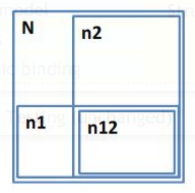
\includegraphics[scale = 0.6]{image/22.PNG}
\end{center}

\vfill\null
\end{multicols}



\newpage
\section{Test execution I}
\textbf{\textit{Describe the principles of scaffolding for test execution. Discuss different types of test oracles. Describe the nature and objectives of unit and integration testing activities. Discuss and compare different integration testing strategies.}}

\subsection{Describe the principles of scaffolding for test execution}
\noindent \textbf{Scaffolding} (échafaud) :
code produced to support development activities especially testing. Not part of the product. May be temporary.\\

\noindent It includes : 
\begin{multicols}{2}
\begin{enumerate}
    \item \textbf{Test
harness}:
environment
in
which
the
component
is
tested.
Ex:
Software
simulation
of
a
hardware
device
    \item \textbf{Test driver}: calls the component. Applies the test cases. A “main” program for running a test
\item \textbf{Test
stubs}:
called
by
the
component.
Substitutes
for
called
components
\end{enumerate}
\vfill\null\columnbreak
\begin{center}
    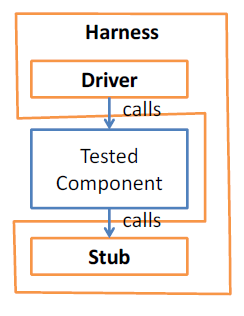
\includegraphics[scale=0.5]{image/45.PNG}
\end{center}
\end{multicols}


\noindent The
scaffolding must
provide : 
\begin{multicols}{2}
\begin{enumerate}
    \item \textbf{Controllability}:
allow to
execute test
cases
    \item \textbf{Observability}:
allow to
judge the
outcome of
tests
    \item [$\Rightarrow$] May
require additional interfaces,
drivers
\end{enumerate}
\vfill\null\columnbreak
\begin{center}
    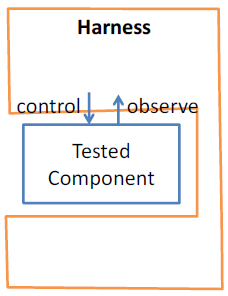
\includegraphics[scale=0.5]{image/46.PNG}
\end{center}
\end{multicols}
\begin{center}
    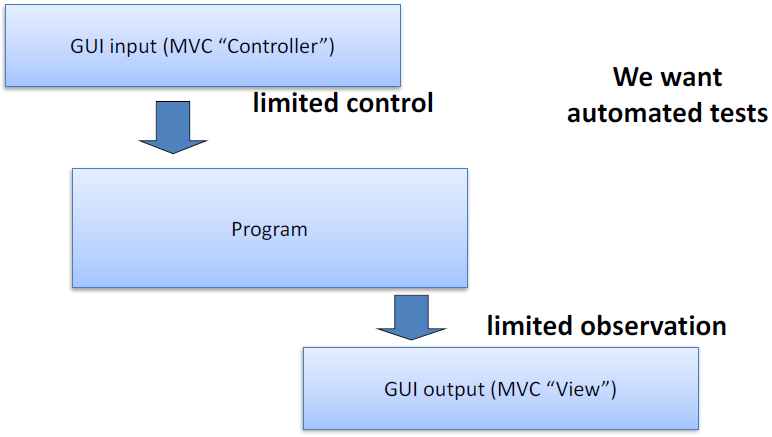
\includegraphics[scale=0.35]{image/47.PNG}
    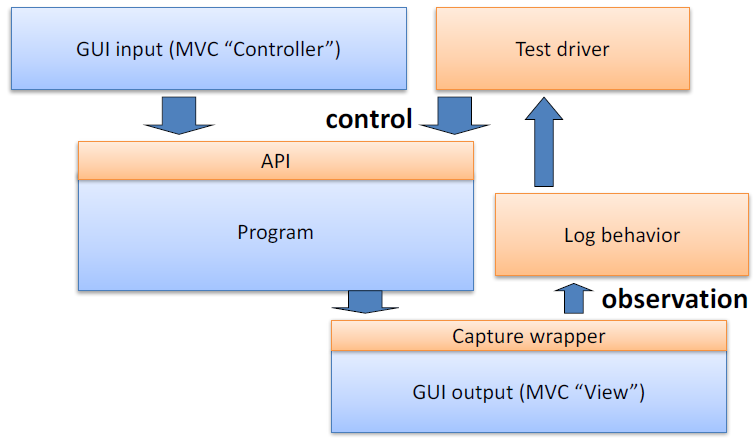
\includegraphics[scale=0.35]{image/48.PNG}
\end{center}

\begin{center}
    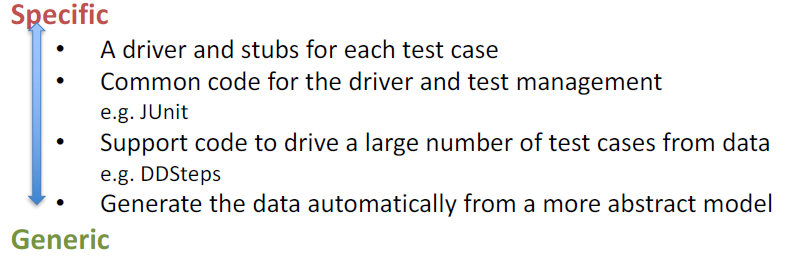
\includegraphics[scale=0.45]{image/49.PNG}
\end{center}



\subsection{Discuss different types of test oracles}
\noindent Did
this
test
case
succeed,
or
fail?
\textbf{Oracle}:
software
that
determines
whether
a
test
passed
or
failed.
\begin{multicols}{2}
\noindent Better
than
manual
checking
\begin{enumerate}
    \item More efficient
    \item More reliable
    \item More capable (e.g timing, large data)\\
\end{enumerate}

\noindent Oracles
should ideally:
\begin{itemize}
    \item [$\bullet$]report
\textbf{PASS} for
\textbf{all} \textbf{correct} executions
    \item [$\bullet$]report
\textbf{FAIL} for
\textbf{all} \textbf{incorrect} executions\\
\end{itemize}

\noindent \textbf{Partial
oracles}:
\begin{itemize}
    \item [$\bullet$]must report PASS for \textbf{all correct} executions
    \item [$\bullet$]may report PASS for \textbf{some} incorrect executions
\end{itemize}
No
false
alarms (FAIL
on
correct
executions). Several partial
oracles
may be more
effective
than one
complete oracle.\\

\noindent \textbf{Comparison‐Based
Oracle} :\\

\begin{center}
    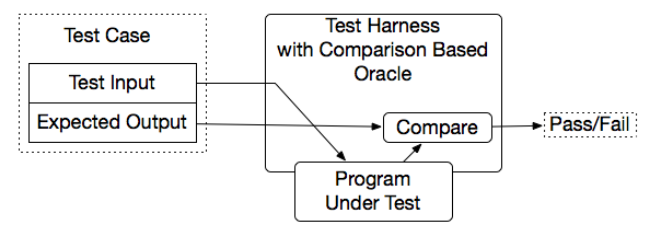
\includegraphics[scale=0.4]{image/50.PNG}
\end{center}

\noindent Oracle
compares
actual
to
expected
output,
reports
if
(actual
=
expected)
then
PASS
else
FAIL.
Fine
for
a
small
number
of
hand‐generated
test
cases. E.g.
JUnit
test
cases:
assertEquals(actual,
expected)\\

\noindent \textbf{Self‐Checks
as
Oracle} :


\begin{center}
    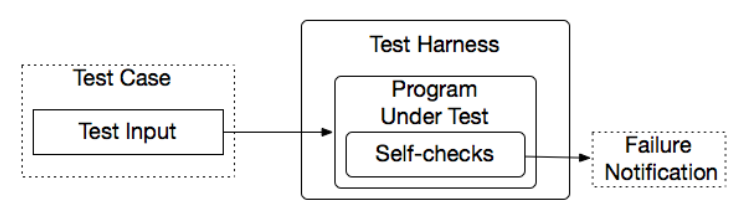
\includegraphics[scale=0.4]{image/51.PNG}
\end{center}


\noindent Oracle as self‐checks in the program (assertions) judge correctness without predicting results
\begin{itemize}
    \item [$+$]Usable with large, automatically generated test suites
    \item [$-$]Often only a partial check. \\
    e.g., structural invariants of data structures\\
\end{itemize}

\noindent Assertions as Oracle :
\begin{itemize}
    \item [$\bullet$]\textbf{Invariants on data structures}\\
    e.g. assert 0 <= size \&\& size <= a.length
    \item [$\bullet$]\textbf{Pre‐ and post‐conditions}\\
    e.g. assert k\makebox{ }!= null; v = dict.get(k); assert dict.contains(k, v);
\end{itemize}
\noindent May
need to
deal
with quantifiers. implement as
iteration $\Rightarrow$ does not
scale well
or
sample some elements (partition
testing!)\\

\noindent \textbf{Capture
and
Replay :}
\begin{center}
    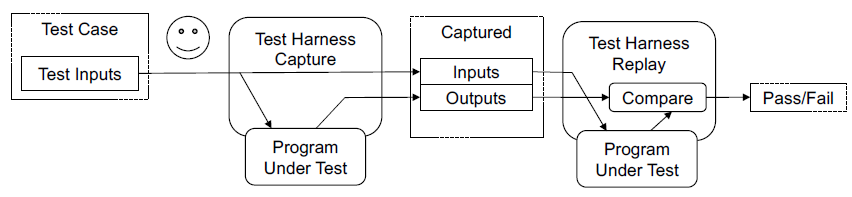
\includegraphics[scale=0.45]{image/52.PNG}
\end{center}
\begin{itemize}
    \item [$\bullet$]\textbf{Capture} a
manually
run
test
case,
sequence
of
inputs,
outputs
    \item [$\bullet$]\textbf{Replay} it
automatically
with
a
comparison‐based
oracle and
compare
actual
to
captured
outputs\\
\end{itemize}
Reusable only until a program change invalidates it. Lifetime depends on abstraction level of input and output.
\vfill\null
\end{multicols}


\subsection{Describe the nature and objectives of unit and integration testing activities}

\begin{center}
    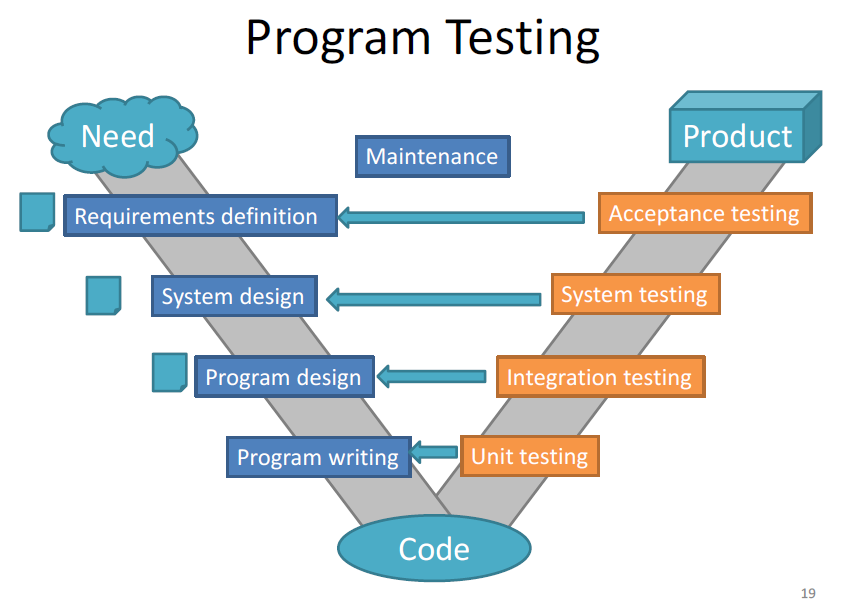
\includegraphics[scale=0.4]{image/53.PNG}
    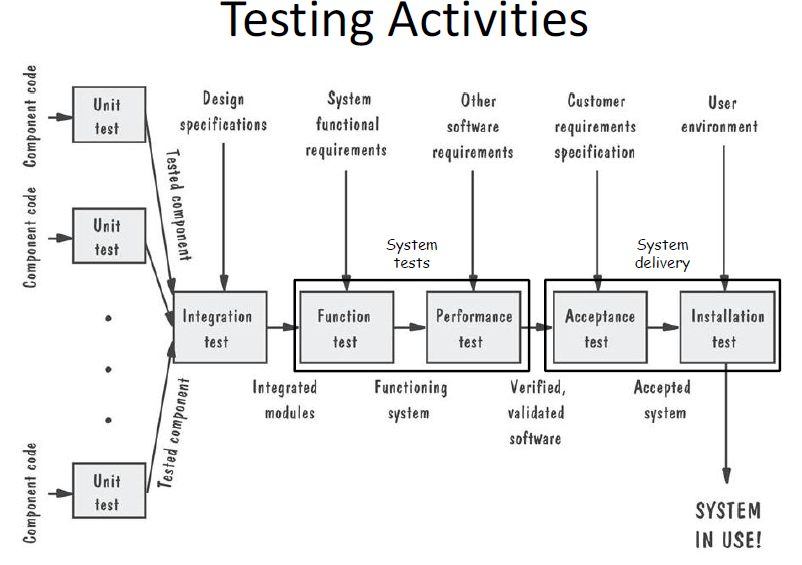
\includegraphics[scale=0.4]{image/54.PNG}
\end{center}

\begin{multicols}{2}
\begin{itemize}
    \item [$\bullet$]\textbf{Unit Testing} : Aka module testing, component testing
    \begin{itemize}
        \item Testing : feed inputs, check valid ouputs
        \item Code reviews, analyses : check internal data structures, logic 
    \end{itemize}
    \item [$\bullet$]\textbf{Integration Testing} : 
    \begin{itemize}
        \item Assemble components together
        \item Check correct interaction
    \end{itemize}
\end{itemize}
\vfill\null
\end{multicols}

\newpage
\subsection{Discuss and compare different integration testing strategies}

\textbf{Structural integration strategies :}
\begin{center}
    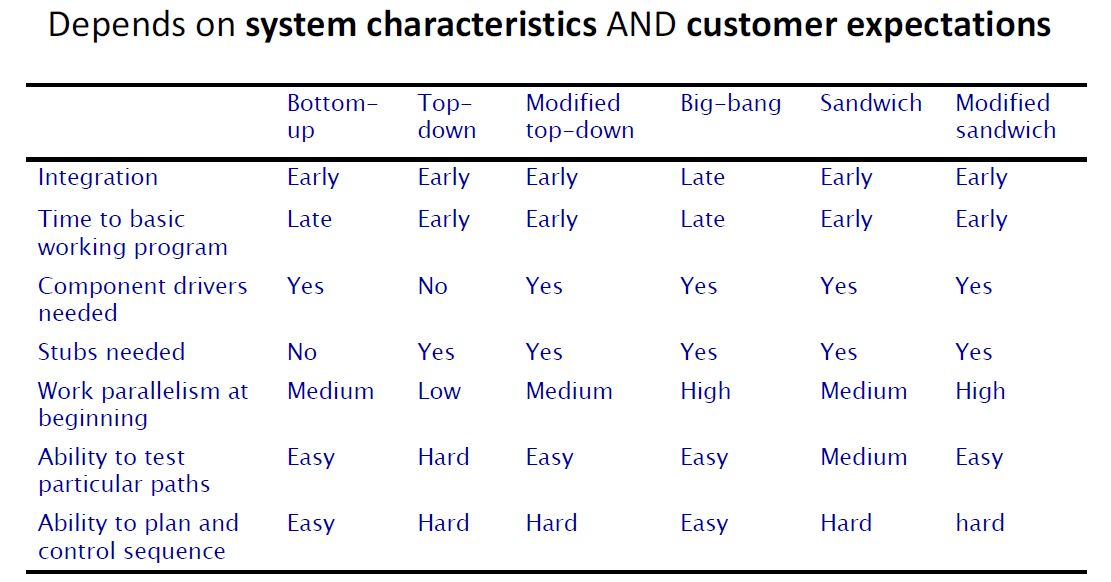
\includegraphics[scale=0.5]{56.PNG}
\end{center}
\textbf{Functional integration strategies :}
\begin{itemize}
    \item \textbf{Threads} : \\
    \textit{Thread} = user-visible program feature across several modules (e.g. send a messages, change user, create mailbox, ...)\\
    Test each thread incrementally.\\
    $\Rightarrow$ Minimizes stubs and drivers but integration plan may be complex.
    \item \textbf{Critical modules} : \\
    Test modules with highest risk first and integrate them with thread or sandwich strategy.\\
    $\Rightarrow$ Requires risk assessment first.\\
\end{itemize}

\newpage
\section{Test execution II}
\textbf{\textit{Describe the nature and objectives of system, acceptance and regression testing activities. Explain regression test selection and prioritization.}}

\subsection{Describe the nature and objectives of system, acceptance and regression testing activities}

\begin{center}
    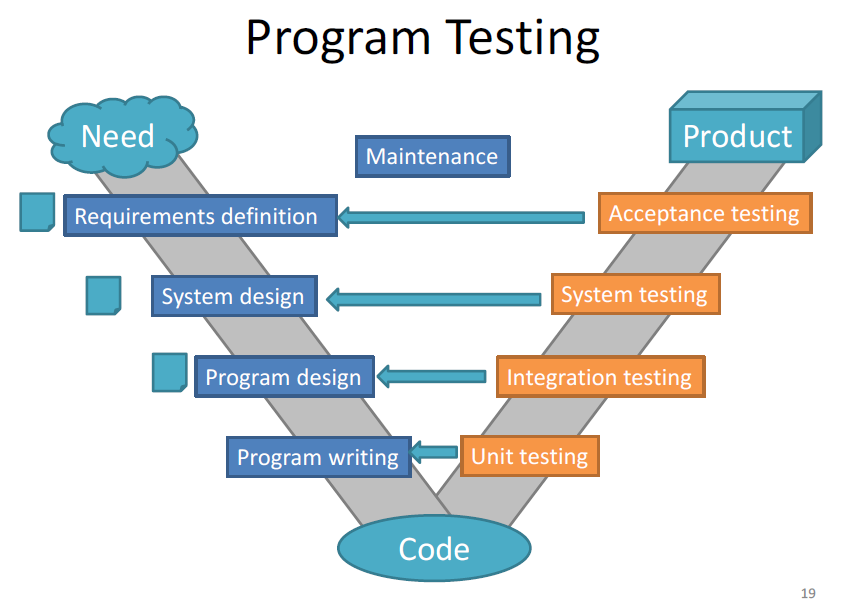
\includegraphics[scale=0.4]{image/53.PNG}
    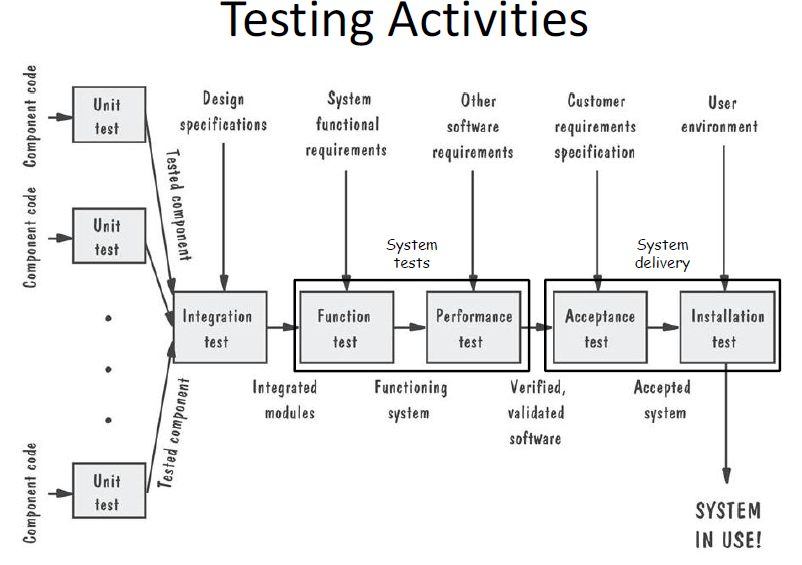
\includegraphics[scale=0.4]{image/54.PNG}
\end{center}

\begin{multicols}{2}
\begin{itemize}
    \item [$\bullet$]\textbf{Function Testing}
    \begin{itemize}
        \item The whole system 
        \item Check that the behaviour conforms to functional requirement specifications
    \end{itemize}
    \item [$\bullet$]\textbf{Performance Testing}
    \begin{itemize}
        \item The whole system 
        \item Check that the behaviour conforms to nonfunctional requirement specifications
    \end{itemize}
    \item [$\bullet$]\textbf{Acceptance Testing}
    \begin{itemize}
        \item The whole system 
        \item Test using the system with the customer
        \item Check that the behaviour conforms to the customer requirement documentation
    \end{itemize}
    \item [$\bullet$]\textbf{Regression Testing}
    \begin{itemize}
        \item Regression =
loss
of
correct
functionality
after
a
change (adding new features; changing, adapting conditions; bugs fixing)
        \item \textbf{Regression
testing =}
re‐executing
tests
after
any
change
to
detect
regressions
        \item Can
be
a
major
cost
of
software
maintenance.
Sometimes
much
more
than
making
the
change
    \end{itemize}
\end{itemize}
\vfill\null
\end{multicols}


\subsection{Explain regression test selection and prioritization}
\noindent Problems of Regression Testing :
\begin{itemize}
    \item Maintaining the test suite (obsolete or redundant tests)
    \item Cost of re-testing = often proportional to the product size
    \begin{itemize}
         \item [$\Rightarrow$]\textbf{Select} or \textbf{prioritize} test cases
    \end{itemize}
\end{itemize}

\begin{multicols}{2}
\noindent \textbf{Test
case
selection:} do
not
execute
some
test
cases.
When
test
cases
are
expensive
to
execute
(special
equipment,
or
long
run‐times,
or
manual
intervention)
\begin{itemize}
    \item [$\bullet$]\textbf{Principle}:
execute
only
test
cases
related
to
elements
that
were
affected
by
the
change\\
    \item [$\Rightarrow$]\textbf{Code‐based
selection}:
only
execute
test
cases
that
execute
changed
or
new
code
\begin{enumerate}
    \item \textbf{Independent}:
a
test
case
can’t
find
a
fault
in
code
it
doesn’t
execute\\
\textbf{Variants}:
changed
CFG
nodes
(control‐flow)
changed
def‐use
pairs
(data‐flow)
    \item Needs
to
record
elements
touched
by
each
test
case
and
modified
by
each
change
\end{enumerate}


    \item [$\Rightarrow$]\textbf{Specification‐based selection}:
only
execute
test
cases
that
test
new
and
changed
functionality\\
Not
independent:
a
test
case
that
is
not
“for”
a
changed
feature
X
might
find
a
bug
in
feature
X\\
$\Rightarrow$ prefer
prioritization rather
than
selection

\end{itemize}

\vfill\null\columnbreak
\noindent \textbf{Test
case
prioritization:}
execute
some
test
cases
less
often.
When
a
very
large
test
suite
cannot
be
executed
every
day
\begin{itemize}
    \item [$\bullet$]\textbf{Basic
idea:}\\
Execute
all test
cases,
eventually
\\Execute
some
sooner
than
others
    \item [$\bullet$]Possible
priority
schemes:
\begin{enumerate}
    \item \textbf{Specification‐based:}
priority
to
test
cases
related
to
changed
and
added
features
    \item \textbf{Round
robin}:
Priority
to
least‐recently‐run
test
cases
    \item \textbf{Track
record:}
Priority
to
test
cases
that
have
detected
faults
before.
They
probably
execute
code
with
a
high
fault
density
    \item \textbf{Structural}:
Priority
for
executing
elements
that
have
not
been
recently
executed\\
Can
be
coarse‐grained:
features,
methods,
files,
...
\end{enumerate}
\end{itemize}
\vfill\null
\end{multicols}


\newpage
\section{Symbolic execution}
\textbf{\textit{Describe the principles of symbolic program execution. Describe the principles of program verification using symbolic execution. Discuss contract-based reasoning on procedures and data structures.}}

\subsection{Describe the principles of symbolic program execution}
Execute the program with symbolic values. Variables receive symbolic values. Execution paths
accumulate symbolic conditions → Bridges program behavior to logic (program behavior becomes logic)
\begin{enumerate}
    \item Values are symbolic expressions

    \item Executing statements computes new expressions
    \item For branching statements, both branches are possible (non-determinism). Need to record the
condition for the execution of each branch
    \item Path accumulate conditions which may become extremely complex. We can simplify it by
replacing a complex condition P with a weaker condition W such that P => W. W describes the
path with less precision (W is a summary of P)
    \item To reason about program behavior in a loop, we can place an invariant. Each time program
execution reaches the invariant W, we can weaken the execution condition P to W:
\begin{enumerate}
    \item check that P => W
    \item substitute W for P
\end{enumerate}
    \item If : 
    \begin{enumerate}
    \item every loop contains an invariant
    \item there is an assertion at the beginning of the program
    \item there is an assertion at the end of the program
\end{enumerate}
Then, every possible execution path is a sequence of segments (basic paths) from one assertion
to the next.
\begin{itemize}
    \item [$\bullet$]\textbf{Precondition}: assertion at the beginning of a segment
    \item [$\bullet$]\textbf{Postcondition}: assertion at the end of the segment
\end{itemize}
\end{enumerate}
%\newpage
\subsection{Describe the principles of program verification using symbolic execution}
\noindent To verify program correctness, we do the following:
\begin{enumerate}
    \item Verify for each basic path:
    \begin{enumerate}
        \item Starting from the precondition
        \item Executing the program segment
        \item The postcondition holds at the end

    \end{enumerate}
    \item Then the execution of any path is correct
\end{enumerate}
\begin{center}
  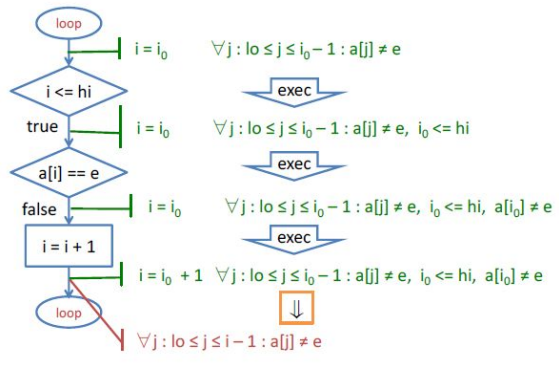
\includegraphics[scale=0.5]{image/23.PNG}  
\end{center}


\subsection{Discuss contract-based reasoning on procedures and data structures}
\begin{multicols}{2}
\begin{itemize}
    \item [$\bullet$]\textbf{On procedure} : Compositional reasoning\\
    Follow the hierarchical structure of a program :
    \begin{itemize}
        \item at a small scale (within a single procedure)
        \item at a larger scales (across multiple procedure ...)

    \end{itemize}
    \textbf{Hoare triple}: [pre] block [post]
    \begin{itemize}
        \item  if pre is satisfied at the entry to the block, then the post should be satisfied after execution of the block
        \item [$\Rightarrow$]summarize the effect of a block of program by a contract [pre] block [post]
        \item [$\Rightarrow$]Prove that block satisfies pre/post then use the contract wherever the block is used
    \end{itemize}

    \vfill\null\columnbreak
    \item [$\bullet$]\textbf{On data structures} :\\
    Data structure module = data (encapsulated) + operations = variables + procedures (methods)\\
    Contract = 
    \begin{enumerate}
        \item \textbf{Abstraction function} "abs" :
relates data structures D to an abstract model abs(D) \\e.g. abs : Dictionary → {<key, value>}
        \item \textbf{Structural invariant} "ok" : data structure characteristics that must be maintained e.g. ok: Dictionary → bool\\
    \end{enumerate}
    Contract for Dictionary.get:
    \begin{lstlisting}
    [<k,v> in abs(dict) and ok(dict)]
    o = dict.get(k)
    [o = v and ok(dict)]
    \end{lstlisting}
\end{itemize}
\end{multicols}


\newpage
\section{Program analysis}
\textbf{\textit{Describe the principles of program inspection, static and dynamic program analysis. Explain symbolic testing and its application to pointer analysis. Explain dynamic analysis and its application to lockset analysis.}}

\subsection{Describe the principles of program inspection, static and dynamic program analysis}
\begin{enumerate}
    \item \textbf{Program inspection} : Systematic,
detailed review of
artifacts (= code
but
also specifications,
documentation,
tests,
...)
to 
find defects and
assess quality.\\ 
Used for : 
\begin{enumerate}
    \item Find and
remove defects
    \item Incentive to
produce good
code
    \item Share
coding norms and
practices
    \item Familiarize new
staff
with the
code\\
\end{enumerate}

\noindent \textbf{Team}:
the
programmer(s)
+
experts (+ usage of \textbf{checklist})\\
with
different
perspectives:
junior
and
senior
engineers,
testers,
managers,
analysts,
architects,
...\\
Moderator:
external
senior
manager
\\
    \item \textbf{Static analysis}: examine source code. Examine the complete execution space but may lead to false
alarm
    \item \textbf{Dynamic analysis}: examine execution traces. No infeasible path problem but cannot examine the
execution space exhaustively
\end{enumerate}

\subsection{Explain symbolic testing and its application to pointer analysis}
\textbf{Symbolic testing} : 
\begin{itemize}
    \item [$\bullet$] abstract variables with \textbf{few symbolic values}
    \item [$\bullet$] apply \textbf{symbolic execution}
    \item [$\bullet$] \textbf{no need} to follow \textbf{all paths}
    \begin{itemize}
        \item explore paths to a limited depth
        \item prune exploration by some criterion
    \end{itemize}
    \item [$\bullet$] sensitivity :
     \begin{itemize}
        \item Symbolic testing is \textbf{path sensitive}: different symbolic states from paths to the same location
        \item Symbolic testing is \textbf{partly context sensitive}: different symbolic states implies different call sequences
        \item This is a strength of symbolic checking
        \begin{enumerate}
            \item detailed description of how fault is reached
            \item costly
            \item reduce costs by memoizing entry and exit conditions
        \end{enumerate}
    \end{itemize}
    \newpage
    \item [$\bullet$] example (\textbf{pointer analysis}): every \textbf{pointer variable} is represented by a \textbf{machine} with three states.\\
    Possible errors: deallocation in \textit{maybe null}, dereference in \textit{maybe null} and dereference in \textit{invalid}.
\end{itemize}
\begin{center}
    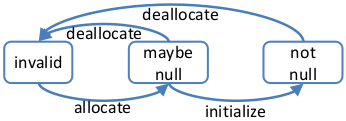
\includegraphics[scale=0.55]{image/pointer_analysis}
\end{center}


\subsection{Explain dynamic analysis and its application to lockset analysis}
\noindent
\textbf{Dynamic program analysis} :
\begin{itemize}
    \item [$\bullet$] track program execution
    \begin{itemize}
        \item instrument program to trace memory accesses
        \item record the state of each memory location
        \item detect accesses incompatible with the current state
        \begin{itemize}
            \item access unallocated memory
            \item read from uninitialized memory
            \item array bounds violations
        \end{itemize}
    \end{itemize}
    \item [$\bullet$] amplify sensitivity of testing to detect potential data races (two threads access a location, and at least one is a write, and there is no lock protecting that location).
\end{itemize}
\vspace{1em}
\textbf{Lockset analysis} :
\begin{itemize}
    \item [$\bullet$]\textbf{Lockset discipline:} Every shared variable must be protected by a lock
    \item [$\bullet$]\textbf{Dynamic lockset analysis}: detects violation of the locking discipline
    \item [$\bullet$]\textbf{Algorithm}:
    \begin{lstlisting}
Identify set of locks held by threads when accessing each shared variable.
For each variable x, a set Lockset(x)
INIT: Lockset(x) = {all locks}
thread A accesses x: Lockset(x) = Lockset(x) $\bigcap$ Locks(A)
END: if Lockset(x) = {} report ERROR (no lock consistently protects v)
    \end{lstlisting}
\end{itemize}
\begin{center}
    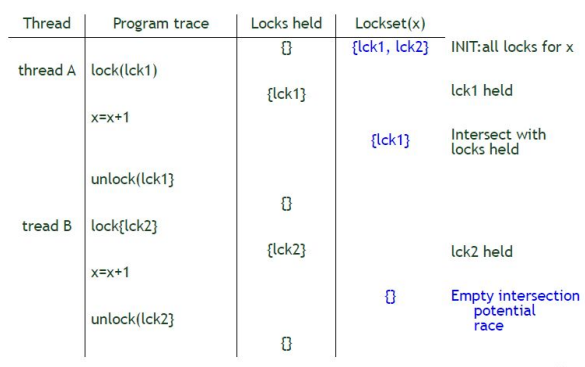
\includegraphics[scale=0.55]{image/24.PNG}
\end{center}

\newpage
\section{Finite state analysis I}
\textbf{\textit{Describe the principles of finite-state analysis. Define safety and liveness properties and discuss their verification. Discuss the model size and correspondence problems.}}

\subsection{Describe the principles of finite-state analysis}
\noindent\textbf{Finite
state
verification:}
\begin{itemize}
    \item [$\bullet$]Prove some significant properties on a finite model of the infinite execution space
    \item [$\bullet$]Techniques from symbolic execution and formal verification
    \item [$\bullet$]Iterative process:
    \begin{enumerate}
        \item Prepare a model and specification
        \item Repeat :
        \begin{enumerate}
            \item Attempt verification
            \item Receive reports of impossible or unimportant faults
            \item Refine the specification and/or the model
        \end{enumerate}
        \item Until no impossible or unimportant faults

    \end{enumerate}
    \item [$\bullet$]Is complementary to testing (can find bugs that are extremely hard to test for [concurrency, race
conditions] but is limited in scope)

\end{itemize}
\subsection{Define safety and liveness properties and discuss their verification}
\vspace*{-0.5cm}
\begin{multicols}{2}
\noindent\textbf{Safety :} 
\begin{itemize}
    \item [$\bullet$]Bad things should not happen\\
    Example :
    \begin{enumerate}
        \item invariant violation, assertion violation
        \item mutual exclusion: two process should not modify a variable at the same time
        \item[3.] [P] S [Q]: partial correctness
    \end{enumerate}
    \item [$\bullet$]Specify with \lstinline{assert(...)}
    \item [$\bullet$]\textbf{Verify with reachability (easy)}
    
\end{itemize}
\begin{center}
    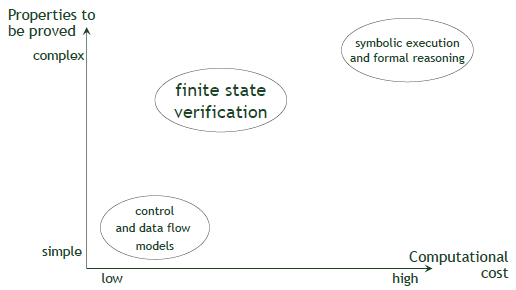
\includegraphics[scale=0.55]{image/25.PNG}
\end{center}
\vfill\null\columnbreak
\noindent\textbf{Liveness :} 
\begin{itemize}
    \item [$\bullet$]Good things should eventually happen\\
    Examples : 
    \begin{enumerate}
        \item response: if I push the button, eventually the
elevator should arrive
        \item fairness: all enabled threads get executed
        \item program termination
    \end{enumerate}
    \item [$\bullet$]Specify in \textbf{temporal logic}
    \begin{center}
    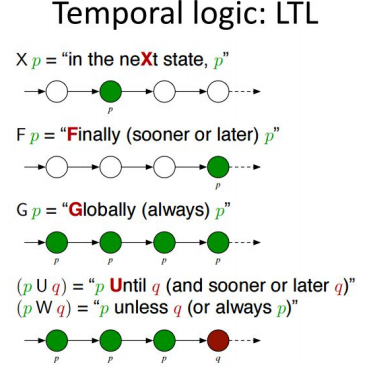
\includegraphics[scale=0.5]{image/26.PNG}
    \end{center}
    \item [$\bullet$]Verify with automata, repeated reachability (more expensive)

\end{itemize}
\end{multicols}


\subsection{Discuss the model size and correspondence problems}
\begin{enumerate}
    \item \textbf{State explosion} : the \textbf{size of the state model} grows very quickly and can become too large.\\
    With \#K processes and \#N states each, the number of global states is : $\#K^{\#N}
\\   $ \item \textbf{Model correspondence problem} : consistency between model and program?
    \begin{enumerate}
        \item \textbf{Model extracted from the program}
        \begin{itemize}
            \item [$\Rightarrow$]verify the \textbf{extraction} procedures (once for all)
            \item [$\bullet$]Challenge: right level of detail
            \begin{enumerate}
                \item all details  $\Rightarrow$ state space explosion
                \item missing details  $\Rightarrow$ “false alarm” reports
            \end{enumerate}
        \end{itemize}
        \item \textbf{Program generated from the model}
        \begin{itemize}
            \item [$\Rightarrow$]verify the \textbf{generation} procedures (once for all)

        \end{itemize}
        Most applicable within well-understood domains
        \item \textbf{Model written (partially or entirely) by hand}
        \begin{itemize}
            \item [$\Rightarrow$]check \textbf{conformance} by (model-based) testing
        \end{itemize}
    \end{enumerate}
    
\end{enumerate}

\newpage
\section{Finite state analysis II}
\textbf{\textit{Explain intensional representations for finite state analysis and describe the use of binary decision diagrams. Discuss iterative model refinement. Describe the principles of data model verification.}}

\subsection{Explain intensional representations for finite state analysis and describe the use of binary decision diagrams}
Enumerating (and storing) all reachable states costs a lot, it is a limiting factor of finite state verification.
The alternative is to use intensional (symbolic) representations which describes sets of reachable states
without enumerating each one individually.
\begin{itemize}
    \item [$\bullet$] Intensional representations may be more compact than the set they represent
    $$\{x\in N | x\; mod \;2 = 0 \wedge 0 < x < 1000  \} \rightarrow 500\; elem$$
    This is only because of structure or regularity in the set that is captured by the representation!

    \item [$\bullet$]Unstructured, irregular sets will necessarily have a larger intensional representation

    \item [$\bullet$]\textbf{Information theory}: representing subsets of N elements ($2^N$ possibilities) requires O(N) in average
\end{itemize}
\vspace{1em}
\textbf{Binary decision diagrams (BDDs)} are a type of intensional model and a compact representation of Boolean functions. A BDD $=$ a binary decision tree with a fixed order on the variables with merged identical subtrees. Operations can be efficiently computed on BDDs.


\subsection{Discuss iterative model refinement}
\noindent Construction of finite state models (balancing
precision and efficiency).\\
Often the first model is unsatisfactory
\begin{itemize}
    \item [$\bullet$]report unfeasible failures
    \item [$\bullet$]exhaust resources before producing any result
    \item [$\Rightarrow$]Idea : improve the model and restart (finite state verification as iterative process)

\end{itemize}

\begin{center}
    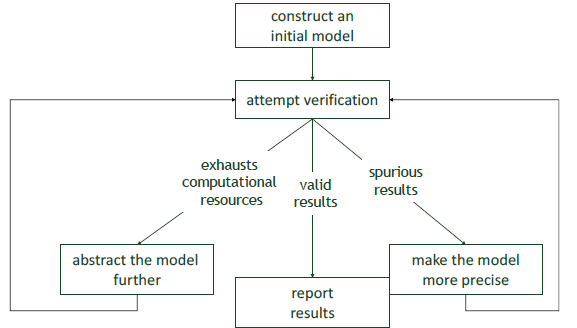
\includegraphics[scale=0.6]{image/27.PNG}
\end{center}

\newpage
\subsection{Describe the principles of data model verification}
\noindent Many information systems are characterized by 
\begin{enumerate}
    \item simple program logic and algorithms
    \item complex data structures
\end{enumerate}
A key element is the data model (class and object diagrams + OCL assertions) = sets of data and
relations among them.\\

\noindent Challenge : prove that 
\begin{enumerate}
    \item individual constraints are consistent

    \item together they ensure the desired properties of the system as a whole\\
\end{enumerate}

\noindent In a complex data models, we use the same general verification principles
\begin{enumerate}
    \item systematic analysis of models

    \item thorough testing is impractical\\
\end{enumerate}
The difficulty is to consider all the possible combinations of choices in a complex data model. (take the
website as an example)


\newpage
\section{Software measurement: size}
\textbf{\textit{State the general principles of software measurement. Discuss size measurement metrics based on lines of code. Explain functional size measurement using function points.}}

\subsection{State the general principles of software measurement}
\noindent \textbf{Principles:}
\begin{itemize}
    \item [$\bullet$]\textbf{Software measurement} : deriving a numeric value of a property of a software product or a process. (To allow comparison)
    \item [$\bullet$]\textbf{Measurement} (more general) : mapping from the empirical world to the formal world.
    \item [$\bullet$]\textbf{Metrics} : a means of measurement of a property of a software product or a process.
    \item [$\bullet$]\textbf{Objective}: understand, control and improve the quality of a software.
    \item [$\bullet$]\textbf{Attributes} :
    \begin{enumerate}
        \item \textbf{Internal} (structural): size, complexity
        \item \textbf{External} (functional) : quality, reliability
    \end{enumerate}
\end{itemize}

\subsection{Discuss size measurement metrics based on lines of code}
\noindent \textit{Note}: A size measurement should be non-negative, zero iff empty and additive.\\

\noindent There are different size metrics: lines of code, number of bytes, number of modules…. The choice of measure is made according to the question to be answered (complexity, disk footprint,...)\\

\noindent \textbf{LOC : Line Of Code} → How to count them? What about blank lines, comments, data declarations,
several instructions on a line
\begin{itemize}
    \item [$\bullet$]\textbf{NCLOC} : No Commented LOC. (No commented line, no blank line, everything else counts as 1 per line)
    \item [$\bullet$]\textbf{CLOC}: Commented LOC. (Line commented)
    \item [$\Rightarrow$]\textbf{LOC} = NCLOC + CLOC
    \item [$\Rightarrow$]\textbf{Comment Density} = CLOC / LOC\\
\end{itemize}
\noindent What count ? What files ? 
\begin{enumerate}
    \item Which files? 
    \begin{itemize}
        \item [$\Rightarrow$]Program code, test drivers, automatically generated code, imported code
    \end{itemize}
    \item Which code? the delivered or the developed?
    \begin{itemize}
        \item [$\bullet$]\textbf{Executable Statement (ES) }: No blank, no comments, no data nor headers, 1 per statement.

        \item [$\bullet$]\textbf{Delivered Source Instruction (DSI)} : No blank, no comment, 1 per statement or data declaration
    \end{itemize}
\end{enumerate}
\newpage
\subsection{Explain functional size measurement using function points}

\noindent \textbf{Function point (FP)}: measures the amount of functionality.\\
Useful to : 
\begin{enumerate}
    \item estimate the development effort and duration (mm/FP)
    \item express defect density (\#defects/FP)
    \item bill the development (\$/FP)\\
\end{enumerate}

\noindent \textbf{Example : Spell-checker spec} \\
The checker accepts as input a document file and an optional personal
dictionary file. The checker lists all words not contained in either of these files. The user can
query the number of words processed and the number of spelling errors found at any stage
during processing.
\begin{multicols}{2}
\begin{itemize}
    \item [$\bullet$]\textbf{Point 1}: Number of items
    \begin{itemize}
        \item  A: external files (file names, menu selection)
        \item B: external output (report message)

        \item  C: external inquiries (interactive inputs requiring a response)
        \item D: external files (interfaces to other systems)

        \item E: internal files (master files in the system)
    \end{itemize}
    \begin{center}
        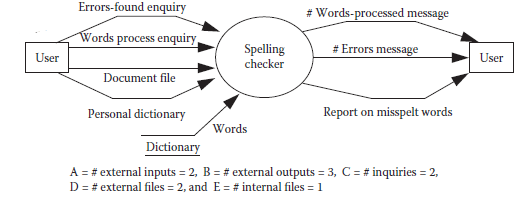
\includegraphics[scale=0.55]{image/28.PNG}
    \end{center}
    \vfill\null\columnbreak
    \item [$\bullet$]\textbf{Point 2}: Complexity for each item (weight)\\
    Unadjusted function points :
    $$UFC = \sum(\#item\;of\;type\;i) * (weight\;of\;type\;i)$$
    \begin{center}
        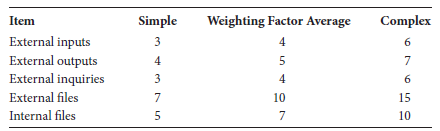
\includegraphics[scale=0.5]{image/29.PNG}
    \end{center}
    Example: all average complexity
    \begin{itemize}
        \item A
=
2,
B
=
3,
C
=
2,
D
=
2,
E
=
1
        \item UFC
=
4
A
+
5
B
+
4
C
+
10
D
+
7
E
=
58\\
    \end{itemize}
    \item [$\bullet$]\textbf{Point 3}: Technical complexity factors (TFC)\\
    Each $F_i$ is between 0 and 5 :
    \begin{itemize}
        \item $TFC = 0.65 + 0.01 \sum F_t$
        \item $FP = UFC * TFC$
    \end{itemize}
    \begin{center}
        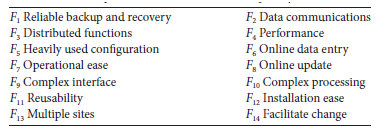
\includegraphics[scale=0.6]{image/30.PNG}
    \end{center}
    Example:
6
factors at
0,
6
factors at
3,
2
factors at
5

\begin{itemize}
    \item TCF
=
0.65
+
0.01
(6
× 3
+
2
× 5)
=
0.93
    \item FP
=
58
× 0.93
=
54
\end{itemize}
\end{itemize}
\end{multicols}

\newpage
\section{Software measurement: structure }
\textbf{\textit{Describe the principles of structure measurement. Describe hierarchical measures based on prime decomposition of control flow graphs. Define cyclomatic complexity measure.
Discuss design-level, inter-modular complexity measures.}}

\subsection{Describe the principles of structure measurement}

The \textbf{size} doesn't tell everything, the \textbf{structure} plays a very important role too to capture the \textbf{complexity}
of the product.
The structure measurement is applicable to design or code seen as a graph. \\

\noindent \textbf{Two perspectives} :  Control Flow \& Data Flow\\

\noindent Structural attributes : 
\begin{enumerate}
    \item \textbf{Complexity} : complicatedness of the connections between elements in a system model (positive, monotonic, additive on disjoints elements)
    \item \textbf{Length} : distance between elements (positive, monotonic, max on disjoints elements)
    \item \textbf{Coupling}: links to/from the elements outside the module (positive, monotonic, at most sum on merged modules)
    \item \textbf{Cohesion}: connections between internal elements (0 to 1, monotonic, at most sum on merged modules)
\end{enumerate}


\subsection{Describe hierarchical measures based on prime decomposition of control flow graphs}
\begin{itemize}
    \item [$\bullet$]\textbf{Control flow graph} : a graph with distinguished start and stop nodes. We want measures that are
independent of a particular view (granularity) of the graph\\

    \item [$\bullet$]\textbf{Prime decomposition}: A structured flow graph can be decomposed into primes (corresponds to a structured program construction). The decomposition is unique, can be done automatically and allows to check whether a program is S-structured (we decompose into primes and we check if all primes are in S).
    Given a family S of prime flowgraphs, a flow graph is S-structured iff it is generated from S by a finite number of sequencing and nesting.

\begin{center}
        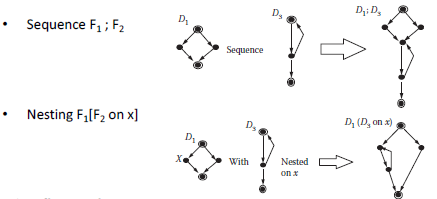
\includegraphics[scale=0.6]{image/31.PNG}
\end{center}

    \item [$\bullet$]\textbf{Prime flow graph}: a graph that cannot be decomposed by sequencing or nesting\\
    \item [$\Rightarrow$]\textbf{Hierarchical measures}: measures defined on the prime decomposition tree. For example: depth of nesting. \\
    More generally:
    \begin{enumerate}
        \item M1: M(F) for each F in S
        \item M2: M($F_1;...;F_n$) from M($F_i$)
        \item M3: M(F($F_1,...,F_n$)) from M($F_i$)
        \item [$\Rightarrow$] M1, M2, M3 gives hierarchical measures (ex: size v(F) $\equiv$ number of nodes)
    \end{enumerate}
\end{itemize}
\newpage

\noindent Example for size v(F) (number of nodes)
\begin{multicols}{2}
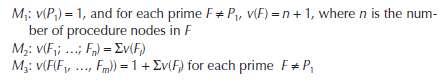
\includegraphics[scale=0.8]{image/32.PNG}

\hspace{1cm}
\includegraphics[scale=0.7]{image/33.PNG}
\end{multicols}
\vspace{-1cm}
\subsection{Define cyclomatic complexity measure}
\begin{itemize}
    \item [$\bullet$]\textbf{Basis set} : a maximal set of linearly independent paths (any path is a linear combination of paths from the basis set)
    \item [$\bullet$]\textbf{Cyclomatic number}: the number of path in a basis set. \\
    $$v(CFG)= \#edges - \#nodes +2 = \#decision points+1$$
    \begin{center}
        \includegraphics[scale=0.6]{image/34.PNG}
    \end{center}
    \item[$\bullet$] Cyclomatic complexity is hierarchical
    \begin{center}
        \includegraphics[scale=0.8]{image/35.PNG}
\end{center}
\end{itemize}


\subsection{Discuss design-level, inter-modular complexity measures}
\noindent So far we have talked about intra-modular measures (inside a procedure). Now we will present
inter-modular measures (dependencies between modules). We thus consider design (module structure
is the same for code).\\
\textbf{Dependency graphs}: graph representing the dependency between modules (information flow or call
graph). Inside modules we have data dependency graphs.
\begin{center}
        \includegraphics[scale=0.4]{36.PNG}
\end{center}


\newpage
\section{Software measurement: quality}
\textbf{\textit{Describe the principles and elements of quality models. Discuss defect-based quality measures. Discuss
usability, maintainability and security measures.}}

\subsection{Describe the principles and elements of quality models}
The question here is: Does a product have desirable attributes? (A product can be a document, a file, a
system,... while an attribute can be completeness, consistency, reliability,...).
Product quality models give a hierarchical nomenclature of product quality characteristics.\\

\noindent A quality models has different elements :
\begin{center}
        \includegraphics[scale=0.65]{37.PNG}
\end{center}


\noindent There are different models such like Boehm or McCall's quality model which are \textbf{fixed models}.
\begin{center}
        \includegraphics[scale=0.6]{38.PNG}
        \includegraphics[scale=0.6]{39.PNG}
\end{center}

\noindent \textbf{But we can also define our own models}:
\begin{itemize}
    \item [$\bullet$]Keep general philosophy of quality models (factors, criteria, metrics)
    \item [$\bullet$]Select attributes suited for a particular product
    \begin{itemize}
        \item [$\blacksquare$]Discuss with customers, users
        \item [$\blacksquare$]Possibly taken from some fixed model
    \end{itemize}
    \item [$\bullet$]Refine to criteria, metrics\\

\end{itemize}
\textbf{We can design it by measurable objectives}:
\begin{itemize}
        \item [$\blacksquare$]Measurable attributes identified in the specification
        \item [$\blacksquare$]Applicable to
small,
evolutionary development,
agile
processes
\end{itemize}
\begin{center}
        \includegraphics[scale=0.7]{40.PNG}
\end{center}

\newpage
\subsection{Discuss defect-based quality measures.}
\noindent We take a narrow view : 
\begin{enumerate}
    \item \textbf{Quality} = lack of defects
    \item \textbf{Defects} = errors, faults, failures
\end{enumerate}
There are known defects (from testing, inspection,...) and latent defects (unknown). 
$$defect\;density = \frac{\#know\;defects}{product\;size}$$

From this equation, one need to define what counts as defects (faults, failures, post-test, post-release,...)
and what counts as size (comments, data binaries, tests,...). It is also important to not confuse with
defect rate which is relative to time and not size.\\

\noindent There are different type of defect-based measures, another example :
$$Spoilage = \frac{time\;to\;fix\;defects}{total\;dev\;time}$$
\subsection{Discuss
usability, maintainability and security measures}
\begin{center}
    \textbf{Usability :}
\end{center}
The degree to which a product or system can be used by specified users to achieve specified
goals with effectiveness, efficiency and satisfaction in a specified context of use.\\

\textbf{Example} : User-friendliness (ease to learn, use, remember) or user satisfaction.\\
$\Rightarrow$ This is not a directly measurable attribute, so we need to define usability measurements
\begin{itemize}
    \item[$\bullet$] \textbf{Effectiveness}: \% of correctly completed tasks. User recall = remember information provided (task effectiveness = quantity x quality of tasks)
    \item[$\bullet$]  \textbf{Efficiency} : time to complete a task, input rate
    \begin{itemize}
        \item[$\blacksquare$] time efficiency = effectiveness / task time
        \item[$\blacksquare$] productive period = productive time / task time
        \item[$\blacksquare$] relative user efficiency = user efficiency / expert efficiency
    \end{itemize}
    \item[$\bullet$] \textbf{Satisfaction} : questionnaires, biological measurements\\
\end{itemize}

\noindent Other usability measurements, not in ISO 25010 :
\begin{itemize}
    \item[$\bullet$] \textbf{Accessibility} : disabilities (visual, hearing, physical)
    \item[$\bullet$] \textbf{Universality} : cultural norms, naming conventions
    \item[$\bullet$] \textbf{Trustfulness}: trust of users in the system ( → security)\\
\end{itemize}

\noindent Internal elements related to usability:
\begin{itemize}
    \item[$\bullet$] good use of menus and graphics
    \item[$\bullet$] informative error messages
    \item[$\bullet$] help functions
    \item[$\bullet$] consistent interfaces
    \item[$\bullet$] well-structured manuals\\
\end{itemize}

\noindent Size and structure can also be measured. In particular, text structure affects readability and
comprehensibility. But size and structure are poor measures of quality.

\newpage
\begin{center}
    \textbf{Maintainability :}
\end{center}
The degree of effectiveness and efficiency with which a product or system can be
modified by the intended maintainers. Easy to understand, enhance and correct. Maintenance can be:
\begin{itemize}
    \item[$\bullet$]Corrective (fix bugs)
    \item[$\bullet$]Adaptive (changes, upgrades)
    \item[$\bullet$]Preventive (before failures occur)
    \item[$\bullet$]Perfective (enhance, extend)\\
\end{itemize}

\noindent They apply to code, documentation, specs, design, tests,... Maintenance is about making changes to the product. There are different maintainability measures :
\begin{itemize}
    \item[$\bullet$](\textbf{Most important one}) \textbf{Mean Time To Repair (MTTR)}: average time to implement a change and restore the system to working order, can be split in different measure times :
    \begin{itemize}
        \item[$\blacksquare$]Problem recognition time
        \item[$\blacksquare$]Administrative delay time
        \item[$\blacksquare$]Maintenance tools collection time
        \item[$\blacksquare$]Problem analysis time
        \item[$\blacksquare$]Change specification time
        \item[$\blacksquare$]Change time (including testing and review) 
    \end{itemize}
    \item[$\bullet$]change time/number of changes
    \item[$\bullet$]number of unresolved problems
    \item[$\bullet$]time spent on unresolved problems
    \item[$\bullet$]\% changes that introduce new faults
    \item[$\bullet$]number of modules modified for a change \\
\end{itemize}

\noindent Concerning internal elements related to maintainability:
\begin{itemize}
    \item [$\bullet$]\textbf{Structural complexity} : this is more an indication, not really a measure. Used in correlation with external measures (e.g. identify a module with poor structure)
    \item [$\bullet$]Readability : for texts, we can use the Fog Index
\end{itemize}

\newpage
\begin{center}
    \textbf{Security :}
\end{center}
The degree to which a product or system protects information and data so that persons or other products or systems have the degree of data access appropriate to their types and levels of authorization.
No “competent programmer” hypothesis: assume that attackers try to overcome security protections and hide their activities.\\

\noindent Security measures :
\begin{enumerate}
    \item \textbf{Risk} = Impact x Likelihood x Threat x Vulnerability (where impact, likelihood and vulnerability depend on threat).
    \item \textbf{Common vulnerability Scoring System (CVSS)} gives a metric between 0 and 1 based on 6 measures. $\textbf{CVSS} = f(AV, AC, Au, C, I, A)$
    \begin{enumerate}
        \item Access vector (AV) : how remote an attacker can be
        \item Access complexity (AC): how complex the attack needs to be
        \item Authentication (Au) : how many authentications needed
        \item Confidentiality impact (C) : impact to system information confidentiality
        \item Integrity impact (I) : impact to system integrity
        \item Availability impact (A) : reduced performance, shutdown
    \end{enumerate}
    \item \textbf{Bayesian analysis (probabilistic)} : based on attack probabilities and costs
    \item \#vulnerabilities / \#defects\\
\end{enumerate}

\noindent \textbf{Internal measures}: Number of entry points, exit points, data channels, persistent data items

\newpage
\section{Software reliability}
\textbf{\textit{Describe the model of reliability based on failure rates. Define failure probability functions, reliability, maintainability, availability, MTTF and MTTR. Describe the case of constant failure rates.}}

\subsection{Describe the model of reliability based on failure rates}

Reliability is a key quality attribute: top-level in all quality models and the most extensively studied.
Reliability has as objectives :
\begin{enumerate}
    \item Measure failures
    \item Predict future failures from past failures
    \item Reliability growth: predict reliability from past faults found and fixed
    \item[$\Rightarrow$]Want to answer a basic question : When will the system fail?
\end{enumerate}


Software failures are different from hardware failures. A component may fail due to
physical wear. The probability that the component will fail at time $t$ is given by the
probability density function $f(t)$

\subsection{Define failure probability functions, reliability, maintainability, availability, MTTF and MTTR}
\begin{itemize}
    \item [$\bullet$]Failure probability \textbf{density function} is the probability that a failure will occur between time t and time t+dt:\\ $f(t)dt=Prob$(failure between t and t+dt)
    \item [$\bullet$]Failure probability \textbf{distribution function} is the probability that a failure will occur between 0 and t: \\
    $F(t)=\int f(t)dt =$ Prob(failure between 0 and t)
    \item [$\bullet$]\textbf{Reliability}: operating without failure for a given time interval. It is time-dependent : \\$R(t) = 1-F(t)$ = Prob(no failure before t)
    \item [$\bullet$]\textbf{Maintainability}: maintenance activity can be carried out within stated time interval, procedures and resources. Also time-dependent:\\ $M(t)$ = Prob(restored before t)
    \item [$\bullet$]\textbf{Availability}: operation without failure at a given point in time, time-independent. \\$A=Prob(not \;failed)= MTTF/(MTTF+MTTR)$
    \item [$\bullet$]\textbf{MTTF}: Mean Time To Failure is the average time before failure occurs. It measures reliability.
    \item [$\bullet$]\textbf{MTTR}: Mean Time To Repair is the average time to fix a fault. It measures maintainability.
\end{itemize}


\subsection{Describe the case of constant failure rates}

\textbf{Constant failure rate}: it is when the software will fail purely randomly independently of the past, no memory.
We have a constant probability rate $\lambda$.
\begin{enumerate}
    \item f(t)= $\lambda$exp(-$\lambda$t)
    \item F(t) = 1-exp(-$\lambda$t)
    \item R(t)= exp(-$\lambda$t)
\end{enumerate}  

\newpage
\section{Failure prediction}
\textbf{\textit{Describe the principles of failure prediction systems. Discuss the example of the Jelinski-Moranda model. Discuss statistical testing.}}

\subsection{Describe the principles of failure prediction systems}

Some basic notions first:
\begin{itemize}
    \item [$\bullet$]Given a series of failure times (t1,t2,...,ti-1) where
the fault has been fixed after each failure. The goal
of these systems is to predict future failure times Ti,
Ti+1,....
    \item [$\bullet$]In software, as we fix faults, we expect the reliability
to grow.
    \item [$\bullet$]The\textbf{ goal of a prediction system} is to predict the probability distributions Fi, Fi+1,...
    \item [$\bullet$]A prediction system has three elements:
    \begin{enumerate}
        \item \textbf{Prediction model}:  probability specification of the stochastic process (distributions Fi(Ti))
        \item \textbf{Inference procedure}: infer unknown parameters of the model from t1,t2,...,tn-1
        \item \textbf{Prediction procedure}: combine the model and inference procedure to make predictions about future
failure behavior
    \end{enumerate}
\end{itemize}

\subsection{Discuss the example of the Jelinski-Moranda model}

\begin{multicols}{2}
\begin{center}
    \includegraphics[scale=0.55]{image/41.PNG}
\includegraphics[scale=0.55]{image/42.PNG}
\end{center}

\end{multicols}

\begin{multicols}{2}
\begin{center}
    \includegraphics[scale=0.55]{image/43.PNG}
\includegraphics[scale=0.55]{image/44.PNG}
\end{center}

\end{multicols}

\newpage
\subsection{Discuss statistical testing}
\textbf{Idea}: reliability predictions based on failures occurring during testing may not correspond to typical system usage (with different users, tasks, experience levels,...).
\begin{enumerate}
    \item Operational Profile: probability distribution on inputs (reflecting usage)
    \item Statistical testing: select tests according to operational profile
    \begin{itemize}
        \item [$\bullet$]Tests focus on more used parts => better observed reliability
        \item [$\bullet$]Test reflects usage => reliability predictions more accurate.

    \end{itemize}
\end{enumerate}


\noindent Operational profiles are difficult to define.\\
$\Rightarrow$ A small \% of the operational profile may account for a large \% of failures.
\noindent Examples:
\begin{enumerate}
    \item Airplane: take-off and landing
    \item Printer : 
    \begin{itemize}
        \item [$\bullet$]non-saturated: available, no queue => print immediately (20\%)
        \item [$\bullet$]saturated: busy, queue => add to queue (79\%)

        \item [$\bullet$]transitional: busy, no queue => create queue and add to queue (1\%)
        \item [$\bullet$]probability of failures: 0.001 per test case
    \end{itemize}
    To have a 50\% chance of detecting each fault, me must run:
    \begin{itemize}
        \item [$\bullet$]non saturated: 2500 test cases
        \item [$\bullet$]saturated: 633 test cases
        \item [$\bullet$]transitional 50 000 test cases
    \end{itemize}
    Transitional likely the most complex and failure-prone !

\end{enumerate}
\end{document}
